%--------------------------- Hoda Abbasi ----------------------------
%----------------------- 10 November 2015 ------------------------

\documentclass[12pt]{book}
\input Latex_macros/Definitionen.tex
\usepackage{a4}
\usepackage[graph]{xy}
\usepackage{graphicx}
\usepackage{tikz-qtree}
\usepackage{latexsym}
\usepackage{amssymb,forest}
\usepackage{tikz}
\usetikzlibrary{arrows}
\setcounter{tocdepth}{4}
\setcounter{secnumdepth}{4}
\usepackage{enumerate}
\usepackage[active]{srcltx}
\usepackage[all]{xy}
\usepackage{xspace}
\usepackage{multicol}
\usepackage{multirow}
\usepackage{caption}
\usepackage{Latex_styles/slashbox}
\usepackage{bussproofs}
\usepackage{xr}
\usepackage{todonotes}
\usepackage{etex}
\usepackage{mathtools} % For \mathmakebox
\newcommand{\Schrift}{report}
   

%%%%%%%%%%%%%%%%%%%%%%%%%%% Symbols %%%%%%%%%%%%%%%%%%%%%%%%%%%%%%%%%%%%%
\DMO{\dhardness}{dys}
\DMO{\nwid}{nwid}

\DMO{\twidth}{tw}
%--------------------------------------------------------------------------------------------------------------------------------------
\begin{document}
\title{\bf \Huge Research Progress Report}

\author{ \bf Hoda Abbasi\\
             PhD Candidate\\
             Computer Science Department\\
             Swansea University\\}
\maketitle
%--------------------------------------------------------------------------------------------------------------------------------------
\tableofcontents
%***************************************************************************************************************************************
%***************************************************************************************************************************************
\chapter{Set Theory}
\label{cha:settheory}
%--------------------------------------------------------------------------------------------------------------------------------------
\section{Ontological Preparations}
\label{sec:Ontological preparations}

A \textbf{thing} is in general fuzzy, perhaps escapes precise definition at all. An \textbf{object} is a clearly defined, clearly outlined 
thing. A \textbf{theory} is about a realm of objects. \textbf{Mathematical objects} are for example various types of numbers and spaces. 
In set theory, every mathematical object is given to us as a \textbf{set}.
%--------------------------------------------------------------------------------------------------------------------------------------
\section{Naive Set Theory}
\label{sec:Naivesettheory}

Pure set theory has exactly one type of object, called ``set'', and thus everything is a set here  \cite{h1}. We find it useful to use an 
extension, where there are ``sets'' and urelements, that is, objects are either urelements (``atomic'') or sets.
\begin{examp}\label{exp:urelemente}
      If we want to assume ``numbers'', like $\NNZ \subset \NN \subset \ZZ \subset \QQ \subset \RR \subset \CC$, then we can consider them 
	  as urelements, that is, they are already given (from the outside), and they have no internal structure, that is, none of these numbers 
	  have elements; compare Section \ref{def:natnumberssimple} for the alternative approach of of defining $\NNZ = \omega$ via sets.
\end{examp}
Intuitively, a set is a ``collection'' of objects, that is, a ``collection'' of sets and urelements. ``Collection'' here means a set $x$ 
(not an urelement), such that for every object $y$ it can be said, whether $y$ is an element of $x$, that is, ``\bmm{y \in x}'', or $y$ is 
not an element of $x$, that is, ``\bmm{y \notin x}''. Thus there is no order on the elements of a set, and an object can not be multiple 
times in a set (it is just ``in or out''). Two objects $x, y$ can be compared for equality, that is, we either have \bmm{x = y} or \bmm{x \ne y}. 
Since a set is given by its elements, we have $x = y$ for sets $x, y$ iff for all objects $z$ holds $z \in x \Lra z \in y$, while we have $x \ne y$ 
iff there is an object $z$ with $z \in x$ but $z \notin y$, or $z \in y$ but $z \notin x$. For an urelement $x$ and every object $y$ holds $y \notin x$. 
Urelements can be compared by equality, where this relation is atomic (given).

\begin{defi}\label{def:sse}
      For sets $x, y$ holds \bmm{x \sse y} if for all objects $z \in x$ holds $z \in y$, while \bmm{x \subset y} holds if $x \sse y$ and $x \ne y$.
\end{defi}

Remarks:
\begin{enumerate}
      \item For any set $x$, we define the \textbf{complement} of $x$, denoted by $x'$, to be the set $x' = \{ z : z \not \in x \}$.
      \item So $x = y$ iff $x \sse y$ and $y \sse x$.
      \item And $x \subset y$ iff for all elements $z \in x$ holds $z \in y$, while there is a $z' \in y$ with $z' \notin x$.
      \item A set $x$ is called a \textbf{proper subset} of a set $y$ if $x \subset y$ but $x \not = y$ \cite{h3}. 
	  \item \cite{h2} uses ``$\subset$'' instead of ``$\sse$''.
\end{enumerate}
%--------------------------------------------------------------------------------------------------------------------------------------
\subsection{Set Formation}
\label{sec:setformation}

Given objects $x, y$ we can form the \textbf{singleton} \bmm{\set{x}} and the \textbf{2-set} \bmm{\set{x,y}}, that is, sets, where for every object $z$ holds:
\begin{enumerate}
      \item $z \in \set{x} \Lra z = x$;
      \item $z \in \set{x,y} \Lra z = x \vee z = y$.
\end{enumerate}

More fundamentally, there is the \textbf{empty set} \bmm{\es}, characterised by the property, that for all objects $x$ holds $x \notin \es$.

Given sets $x, y$, we can form three further sets:
\begin{itemize}
      \item the \textbf{union} \bmm{x \cup y}, characterised by $\fa\, z : z \in x \cup y \Lra z \in x \vee z \in y$;
      \item the \textbf{intersection} \bmm{x \cap y}, characterised by $\fa\, z : z \in x \cap y \Lra z \in x \wedge z \in y$;
      \item the \textbf{(set-)difference} \bmm{x \sm y}, characterised by $\fa\, z : z \in x \sm y \Lra z \in x \wedge z \notin y$.
\end{itemize}
Remarks:
\begin{enumerate}
      \item Intersection and union operation are {\it commutative} and {\it associative}.
      \item For sets $x, y, z$ we have the following properties \cite{h1}.
      \begin{enumerate}
            \item $x - \emptyset = x\ ;\ x - x = \emptyset $. 
            \item $x \cup x = x\ ;\ x \cap x = x $.
            \item $x \subseteq x \cup y\ ;\ x \cap y \subseteq x$.
            \item $x \cup (y \cap z) = (x \cup y) \cap (x \cup z)$.
            \item $x \cap (y \cup z) = (x \cap y) \cup (x \cap z)$.
            \item $(x \subseteq y) \leftrightarrow (x \cap y=x) \leftrightarrow (x \cup y = y)$.
            \item $x - y = x - (x \cap y)$.
      \end{enumerate}
      \item Two sets are said to be \bmm{disjoint} if they have no member in common; in symbols \cite{h1},
      $$ x \cap y = \emptyset .$$
      \item  For sets $x, y$ the \textbf{De Morgan's Laws} are:
	  \begin{enumerate}
	        \item $ ( x \cup y)' = x' \cap y' $;
			\item $ ( x \cap y)' = x' \cup y' $.
	  \end{enumerate}
	  \item If $x, y $ are subset of $z$ , we have the following properties:
      \begin{enumerate}
	        \item $z - ( z - x ) = x$;
	        \item $(x \subseteq y) \leftrightarrow [(z - y) \subseteq (z - x)]}$;
	        \item $x \cup (z - x) = z$;
	        \item $z - (x \cup y) = (z - x) \cap (z - y)$;
	        \item $z - (x \cap y) = (z - x) \cup (z - y)$.
	  \end{enumerate}
      \item From the {\it axiom of extensionality}, it is proved that there is only one empty set \cite{h1}.
\end{enumerate}
%--------------------------------------------------------------------------------------------------------------------------------------
\subsection{(Ordered) Pairs}
\label{sec:ordpairs}

\begin{defi}\label{def:pairs}
      For objects $x, y$ we define the \textbf{pair} \bmm{(x,y)} via
      \begin{displaymath}
            (x,y) := \set{\set{x},\set{x,y}}.
      \end{displaymath}
      A set $x$ is called \textbf{a pair}, if there are objects $y,z$ with $x = (y,z)$.
\end{defi}
Remarks:
\begin{enumerate}
      \item If $x=y$, then $(x,y) = \set{\set{x}}$.
      \item For example, $\es$ is not a pair.
\end{enumerate}
\begin{lem}\label{lem:pairs}
      For objects $x, y, x', y'$ holds $(x,y) = (x',y') \Lra x = x' \wedge y = y'$.
\end{lem}
\begin{defi}\label{def:projpairs}
      For a pair $x$ we define the object \bmm{\proj_1(x)}, \bmm{\proj_2(x)} as those unique objects with $x = (\proj_1(x), \proj_2(x))$ (``projections'').
\end{defi}

%--------------------------------------------------------------------------------------------------------------------------------------
\subsection{Binary Operation}
\label{sec:Binary Operation}

\begin{defi}\label{def:bop}
      The \textbf{binary operation $P$} or \textbf{law of composition} on a set $x$ is the set 
	  $$ \{ (a,b) \mid a \in x \wedge b \in x \wedge P(x,y) \}.$$
\end{defi}
In other words, the binary operation on set $x$ is a rule which for every two elements of $x$ gives another element of $x$.
For example, addition is a binary operation on $\RR$, because given any two real numbers, their sum is a real number.
If $R$ is a binary relation on a set $x$, we write $ \bmm{R(a,b)}$ or $\bmm{(aRb)}$ \cite{h1}.
%--------------------------------------------------------------------------------------------------------------------------------------
\subsection{Product of Sets}
\label{sec:productsets}

\begin{defi}\label{def:productsets}
  For sets $X, Y$ the set of all pairs $x, y$ with $x \in X$ and $y \in Y$ exists and is denoted by
  \begin{displaymath}
    \bmm{X \times Y} := \set{(x,y): x \in X \wedge y \in Y}.
  \end{displaymath}
\end{defi}
Remarks:
\begin{enumerate}
      \item For sets $A, B, C, D$ we have the following properties.
      \begin{enumerate}
            \item\label{thm:propprod5} $A \times \emptyset = \emptyset \times A = \emptyset$.
            \item\label{thm:propprod1} $A \times (B \cap C) = (A\times B) \cap (A \times C)$.
            \item\label{thm:propprod2} $A \times (B \cup C) = (A \times B) \cup (A \times C)$.
            \item\label{thm:propprod3} $(A \times B) \cap (C \times D) = (A \cap C) \times (B \cap D)$.
            \item\label{thm:propprod4} $(A \times B) \cup (C \times D) \subseteq (A \cup C) \times (B \cup D)$.
      \end{enumerate}
\end{enumerate}
%--------------------------------------------------------------------------------------------------------------------------------------
\subsection{Infinitary Set Constructions}
\label{sec:Infinitary set constructions}

\begin{itemize}
      \item A \textbf{set system} is a set $X$, such that for all $y \in X$ holds that also $y$ is a set (all elements are sets). For a set system 
	  $X$ the \textbf{union} \bmm{\bc X} is characterised by $x \in \bc X \Lra \ex\, y \in X : x \in y$.
      \item For a set $x$ there is the \textbf{power set} \bmm{\pot(x)}, characterised by $y \in \pot(x) \Lra y \sse x$ for sets $y$ (the power set 
	  is the set of all subsets). So a powerset is a set system.
      \item If $x$ is a set, and $\Phi(y)$ a property of a set variable $y$ (a logical formula), then $\set{y \mb y \in x \wedge \Phi(y)}$ is a set, 
	  characterised by the property, that the elements of it are precisely those $y$ with $y \in x$ and $\Phi(y)$. In this way we can form specific 
	  subsets (via \textbf{comprehension}).
      \item If $X$ is a set, and $F(x)$ a specification of a unique object for all $x \in X$, then we have the set $\set{F(x) \mb x \in X}$, which 
	  is the set of all objects $y$, such that there is some $x \in X$ with $y = F(x)$. This is a form of image (via \textbf{replacement}).
\end{itemize}

\begin{examp}\label{exp:infset}
      For set $A= \{1,2\}$ the power set is : $\pot(A)=\{ \emptyset,\{1\},\{2\},\{1,2\}\}$.
\end{examp}
%--------------------------------------------------------------------------------------------------------------------------------------
\subsection{Relations and Maps}
\label{sec:maps}

\begin{defi}\label{def:reli}
      A \textbf{relation} is a set of pairs. The \textbf{first projection} of a relation $R$ is $\bmm{\proj_1(R)} := \set{\proj_1(p) : p \in R}$, 
	  the \textbf{second projection} is $\bmm{\proj_2(R)} := \set{\proj_2(p) : p \in R}$. For a relation $R$ and a set $X$ one defines 
	  $\bmm{R(X)}:= \set{y \in \proj_2(R) \mb \ex\, x \in X : (x,y) \in R}$ (the ``image'' of $X$ under $R$).
\end{defi}

\begin{defi}\label{def:reli2}
      A relation is \textbf{well-defined} if each element in the domain is assigned to a unique element in the range.
\end{defi}	  
Remarks:
\begin{enumerate}
      \item Instead of ``second projection'' one might also use ``range''. However for the first projection to use ``domain'' is misleading, since 
	  a relation does not need to have every element of the domain in its first projection (different from a map).

      The notations $\proj_i(R)$ for $i \in \tb{1,2}$ can be understood as a special case of the notation ``$R(X)$'', but where $R$ is not a set.
      \item $\es$ is a relation, and for all sets $X$ holds $\es(X) = \es$.
\end{enumerate}

\begin{defi}\label{def:binop}
      For any binary relation on a set $x$ we say:
	  \begin{itemize}
	        \item $R$ is \textbf{reflective} if $ (\forall a \in x) \ ( aRb)$;
			\item $R$ is \textbf{symmetric} if $ (\forall a,b \in x) \ ( aRb \rightarrow bRa)$;
			\item $R$ is \textbf{antisymmetric} if $ (\forall a,b \in x) [ ( aRb \wedge a \not = b)\rightarrow \neg (bRa)]$;
			\item $R$ is \textbf{connected} if $ (\forall a,b \in x) [(a \not = b) \rightarrow (aRb \vee bRa)]$;
			\item $R$ is \textbf{transisive} if $ (\forall a,b,c \in x) [ ( aRb \wedge bRc) \rightarrow (aRc)]$ \cite{h1}.
	  \end{itemize}
\end{defi}

A binary relation on a set is said to be an \textbf{equivalence relation} just in the case it is reflexive, symmetric and transisive \cite{h1}.

\begin{defi}\label{def:map}
      A \textbf{map} is a relation $f$ such that for all $x \in \proj_1(f)$ there is exactly one $y \in \proj_2(F)$ with $(x,y) \in f$, where then 
	  $y =: \bmm{f(x)}$ is used. Furthermore $\bmm{\dom(f)} := \proj_1(f)$ (``domain'') and $\bmm{\rg(f)} := \proj_2(f)$ (``range'').
\end{defi}
Remarks:
\begin{enumerate}
      \item Normally there is no confusion between $f(X) = \set{f(x) : x \in X \cap \dom(f)}$ for a set $X$ according to Definition \ref{def:reli}, 
	  and $f(x) = y$ for a \emph{single} argument $x \in \dom(f)$.
\end{enumerate}
%--------------------------------------------------------------------------------------------------------------------------------------

\subsection{Special Maps}
\label{sec:Specialmaps}

\begin{defi}\label{def:inj}
      A map $f$ is called an \textbf{injection} (is ``injective'' or ``one-to-one'') if for all $x, x' \in \dom(f)$ holds $f(x) = f(x') \Ra x = x'$.
\end{defi}
\begin{defi}\label{def:surj}
      For a map $f$ holds the statement \bmm{f:X \ra Y} if $X, Y$ are sets with $X = \dom(f)$ and $\rg(f) \sse Y$. Such a statement attaches to 
	  \textbf{codomian} (or ``target set'') $Y$ to the map $f$. Given such a codomain $Y$, $f$ is called \textbf{surjective} or ``onto'' if $\rg(F) = Y$.
\end{defi}
\begin{defi}\label{def:bij}
      A map $f$ with codomain $Y$ is called \textbf{bijective} (``is a bijection'') if $f$ is injective and surjective.
\end{defi}
Remarks:
\begin{enumerate}
      \item If sets $A , B$ are injective and infinite, then $\abs{A} \leq \abs{B}$
\end{enumerate}
\begin{examp}\label{exp:Specialmaps1}
      For map $f: \NN \to \NN$ and $f=2x$, the codomain is $\NN$ but the range is even numbers.
\end{examp}

\begin{examp}\label{exp:Specialmaps2}
      The map $F(x) = 3 x + 7$ is injective but the map $G(x) = x^4 - x$ is not.
\end{examp}

\begin{examp}\label{exp:Specialmaps3}
      Fig \ref{fig:injct} showes an examples of injective and non-injective maps. 
	  Fig \ref{fig:bijct} showes an examples of bijective and non-bijective maps.
	  \begin{figure}
      \begin{center}
	  %\centering
      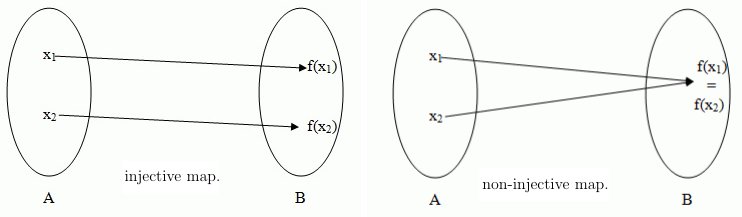
\includegraphics[scale =0.8]{p11.png}
      \caption{Examples of injective and non-injective maps.}
	  \label{fig:injct}
      \end{center}
      \end{figure}
	  %----------
	  \begin{figure}
      \begin{center}
	  %\centering
      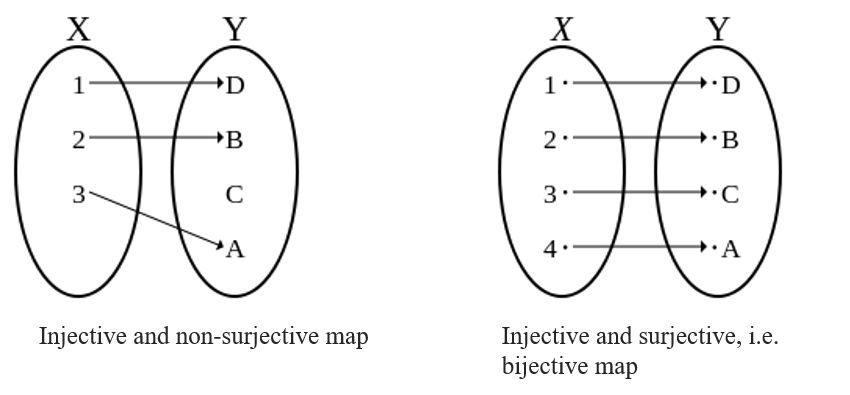
\includegraphics[scale =0.8]{p5.png}
      \caption{Examples of bijective and non-bijective maps.}
	  \label{fig:bijct}
      \end{center}
      \end{figure}
\end{examp}

\begin{examp}\label{exp:Specialmaps4}
      The map $F(x) = 2 x $ from natural numbers to the set of non-negative even numbers is surjective but from the set of natural numbers 
	  to natural numbers is non-surjective.
\end{examp}
\begin{examp}\label{exp:Specialmaps5}
      The map $F(x) = x^2$ from the set of positive numbers to positive real numbers is injective and surjective. Therefore, it is bijective.
\end{examp}
%\begin{figure}
       %\begin{center}
	   %\centering
       %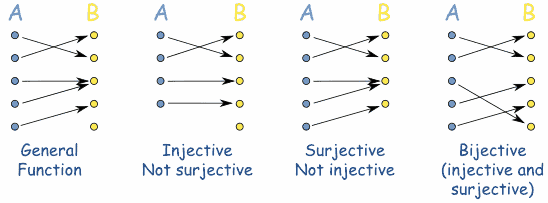
\includegraphics{p3.png}
       %\caption{Example of different typs of map.}
       %\end{center}
%\end{figure}
%--------------------------------------------------------------------------------------------------------------------------------------
\subsection{Decompositions and Equivalence Relations}
\label{sec:Decompositions}

\begin{defi}\label{def:Decompositions}
      A \textbf{partition} of a set $X$ is some $P \sse \pot(X) \sm \set{\es}$ wich is disjoint, i.e., $\fa\, A, B \in P : A \ne B \Ra A \cap B = \es$, 
	  and where $\bc P = X$.
\end{defi}
\begin{examp}\label{exp:Decompositions}
      The set $X = \{ 1, 2, 3 \} $ has these five partitions:
      $$ \{ \{1\}, \{2\}, \{3\}\}$$
      $$ \{ \{1,2\}, \{3\}\}$$
      $$ \{ \{1, 3\}, \{2\}\}$$
      $$ \{ \{1\}, \{2, 3\}\}$$
      $$ \{ \{ 1, 2, 3 \}\}$$
      The following are not partitions of X.
      $$ \{ \{\}, \{2, 3\}\}$$
      $$ \{ \{1, 2\}, \{2, 3\}\}$$
      $$ \{ \{1\}, \{2\}\}$$
\end{examp}

\begin{examp}\label{exp:partition}
      $\ZZ$ can be partitioned into three disjoint subset as follows:
	  $$ \{3k \mid k \in \ZZ\}, \{3k+1 \mid k \in \ZZ\}, \{3k+2 \mid k \in \ZZ\}$$
\end{examp}
%--------------------------------------------------------------------------------------------------------------------------------------
\subsection{Finite Sets}
\label{sec:Finite sets}

\begin{defi}\label{def:finite}
      A set $X$ is called \textbf{infinite} if there is a bijection $f: X \ra X'$ for some $X' \subset X$, otherwise $X$ is called \textbf{finite}.
\end{defi}
\begin{defi}\label{def:finitesubs}
      For a set $X$ let $\bmm{\pote(X)} := \set{S \in \pot(X) : S \text{ finite}}$ be the set of finite subsets of $X$.
\end{defi}
\begin{lem}\label{lem:finitesubs}
      For a set $X$ holds $\pot(X) = \pote(X)$ iff $X$ is finite.
\end{lem}
%--------------------------------------------------------------------------------------------------------------------------------------
\subsection{Natural Numbers}
\label{sec:natnumbers}

\begin{defi}\label{def:natnumberssimple}
      We can define the first \textbf{natural numbers} as $\bmm{0} := \es$, $\bmm{1} := \set{0}$, $\bmm{2} := \set{0,1}$, $\bmm{3} := \set{0,1,2}$.
\end{defi}
	  \begin{defi}\label{def:successor}
      In general, we can define the \textbf{successor} of a set $x$ as $\bmm{x'} := \set{x} \cup x$. So $1 = 0'$, $2 = 1'$, $3 = 2'$, and so on.
\end{defi}
Remarks:
\begin{enumerate}
      \item An important axiom of set theory is the \textbf{axiom of infinity}, which can be stated as the statement, that there is a set $X$ with
	  $\es \in X$ and $\fa\, x \in X : x' \in X$.
	  \item A nonempty subset $S$ of $\ZZ$ is  \textbf{well-ordered} if $S$ contains a least element. The set $\ZZ$ is not well-ordered since it does not 
	  contain a smallest element. However, the natural numbers are well-ordered.
	  \item \textbf{Principle of Well-Ordering}: Every nonempty subset of the natural numbers is well-ordered.
\end{enumerate}

\begin{lem}\label{lem:omega}
      There exists a smallest set $\omega$ with $\es \in \omega$ and $\fa\, x \in \omega : x \in \omega \Ra x' \in \omega$, that is, $\omega$ is 
	  the unique set with these two properties and the condition, that for every set $X$ with these two conditions we have $\omega \sse X$.
\end{lem}
Remarks:
\begin{enumerate}
      \item We use $\omega$ for the set of natural numbers including zero, if we wish to use the concrete representation of natural numbers, otherwise 
	  we use \bmm{\NNZ}, and $\bmm{\NN} := \NNZ \sm \set{0}$.

      So we can define $\NNZ := \omega$, but when using this notation, then we do not make use of the internal structure of natural numbers 
	  so we might consider them as urelements).
\end{enumerate}
%--------------------------------------------------------------------------------------------------------------------------------------
\subsection{The Size of Sets}
\label{sec:sizeofsets}

\begin{defi}\label{def:equalsize}
      Two sets $X, Y$ \textbf{have the same size}, if there exists a bijection from $X$ to $y$.
\end{defi}
\begin{lem}\label{lem:sizefiniteset}
      A set $X$ is finite if and only if there is $n \in \omega$ such that $X$ has the same size as $n$, and where $n$ is uniquely determined.
\end{lem}
\begin{defi}\label{def:sizefiniteset}
      For a finite set $X$ by $\bmm{\abs{X}} \in \omega$ we denote the unique $n \in \omega$ with the same size as $X$ (according to Lemma 
	  \ref{lem:sizefiniteset}).
\end{defi}
Remarks:
\begin{enumerate}
      \item For the sets $A , B$, we have the following properties:
      \begin{enumerate}
            \item $\abs{A \times B }= \abs{A} \times \abs{B}$.
	        \item If $\abs{A} = n$ then $\abs{\pot(A)} = 2^n$.
	        \item $\abs{A \cup B} = \abs{A} + \abs{B} - \abs{A \cap B}$.
      \end{enumerate} 
\end{enumerate}
%--------------------------------------------------------------------------------------------------------------------------------------
%***************************************************************************************************************************************
%***************************************************************************************************************************************
\chapter{Brief Introduction to Abstract Algebra}
\label{cha:Abstract Algebra}

%--------------------------------------------------------------------------------------------------------------------------------------
%\subsection{Matrix}
%\label{sec:Matrix}

%--------------------------------------------------------------------------------------------------------------------------------------
\section{Group}
\label{sec:Group}

\begin{defi}\label{def:group1}
      A \textbf{group} is a pair $(G,\circ)$ where $G$ is a set and $\circ$ is a binary operation on $G$, such that the following four properties hold
	  \begin{enumerate}
	        \item (\textbf{closure}) for all $a, b \in G, a \circ b \in G$;
			\item (\textbf{associativity}) for all $a, b, c \in G, a \circ (b \circ c) = (a \circ b) \circ c$;
			\item (\textbf{existence of the identity element}) there is an element $e \in G$ such that for all $a \in G, a \circ e = e \circ a = a$;
			\item (\textbf{existence of inverses}) for every $a \in G$, there is an element $b \in G$ (called the inverse of $a$) such that
            $a \circ b = b \circ a = e$.
	  \end{enumerate}
\end{defi}

\begin{examp}\label{exp:group1}
      $(\RR,+)$ is a group. We know already that addition is a binary operation on $\RR$, so ‘closure’ holds. We know addition of real numbers
       is associative. We want an element $e \in \RR$ so that $a + e = e + a = a$ for all $a \in \RR$. It is clear that $e = 0$ works and 
	   is the only possible choice. Moreover, the (additive) inverse of $a$ is $-a : a +(-a) = (-a) + a = 0$.
\end{examp}

\begin{examp}\label{exp:group2}
      $(\RR^2,+)$ is a group. Since the  elements of $\RR^2$ are pairs $(a_1,a_2)$ where $a_1, a_2$ are real numbers. Addition is defined
      by 
      $$(a_1,a_2)+(b_1,b_2) = (a_1+b_1,a_2+b_2).$$
      Note that the entries $a_1 + b_1$ and $a_2 + b_2$ are real numbers, and so $(a_1 + b_1,a_2 +b_2)$ is a pair of real numbers. Hence 
	  $(a_1 + b_2,a_2 + b_2)$ is in $\RR^2$ (closure). It can be proved that other laws (associativity, existence of the identity element 
	  and exictence of inverse) are satisfied.
\end{examp}

\begin{defi}\label{def:group2}
      A group $(G,\circ)$ is called \textbf{abelian} if it satisfies (\textbf{commutativity}) for all $a, b \in G, a \circ b = b \circ a$.
\end{defi}

\begin{examp}\label{exp:group3}
      These are some examples of abelian groups: 
	  $$(\RR,+), (\CC,+), (\QQ,+), (\RR^n,+).$$
\end{examp}
\begin{defi}\label{def:group3}
      Let $(G,\circ)$ be a group. Let $H$ be a subset of $G$ and suppose that $(H,\circ)$ is also a group. Then we say that $H$ is a 
	  \textbf{subgroup} of $G$ (or more formally $(H,\circ)$ is a subgroup of $(G,\circ)$). 
\end{defi}	  
For $H$ to be a subgroup of $G$, we want $H$ to a group with respect to the same binary operation that makes $G$ a group.

\begin{examp}\label{exp:group4}
      $\ZZ$ is a subgroup of $\RR$ (or more formally, $(\ZZ,+)$ is a subgroup of $(\RR,+)$); because Z is a subset of $R$ and both are
	  groups with respect to the same binary operation which is addition.
\end{examp}

\begin{examp}\label{exp:group5}
      The set $V = \{(a,a) : a \in \RR \}$ is the line $y = x$. It contains the identity element $(0, 0)$, is closed under addition
      and negation. Therefore it is a subgroup of $\RR^2$.
\end{examp}

\begin{examp}\label{exp:group6}
      The ray $W = \{(a,a) : a \in \RR, a \geq 0 \}$ is not a subgroup of $\RR^2$. It contains the identity element $(0,0)$ and
      is closed under addition. The problem is with the existence of additive inverses; e.g. $(1,1)$ is in $W$ but its inverse
      $(-1,-1)$ is not in $W$.
\end{examp}

\begin{lem}\label{lem:sizefiniteset}
      Let $G$ be a group. A subset $H$ of $G$ is a subgroup if and only if it satisfies the following three conditions:
      \begin{enumerate}
	        \item $1 \in H$,
		 	\item if $a, b \in H$ then $ab \in G$,
		 	\item if $a \in H$ then $a^-^1 \in H$.
	   \end{enumerate}
\end{lem}
	 
\begin{defi}\label{def:group4}
      The \textbf{order} of an element $a$ in a group $G$ is the smallest positive integer $n$ such that $a^n =1$. If there is no 
	  such positive integer $n$, we say a has \textbf{infinite order}.
\end{defi}
%--------------------------------------------------------------------------------------------------------------------------------------
\section{Ring}
\label{sec:Ring}

\begin{defi}\label{def:ring1}
      A \textbf{ring} is a triple $(R,+, \cdot)$, where $R$ is a set and $+, \cdot$ are binary operations on $R$ such that the following properties hold:
      \begin{enumerate}
	         \item (closure) for all $a, b \in R, a + b \in R$ and $a \cdot b \in R$;
			 \item (associativity of addition) for all $a, b, c \in R, (a+b) +c = a +(b+c)$;
			 \item (existence of an additive identity element) there is an element $0 \in R$ such that for all $a \in R, a + 0 = 0 + a = a$.
			 \item (existence of additive inverses) for all $a \in R$, there an element, denoted by $-a$, such that $a +(-a) = (-a)+ a = 0$;
			 \item (commutativity of addition) for all $a, b \in R, a + b = b +a$;
			 \item (associativity of multiplication) for all $a, b, c \in R, a \cdot (b \cdot c) = (a \cdot b) \cdot c$;
			 \item (distributivity) for all $a, b, c \in R, a \cdot (b + c) = a \cdotb + a \cdot c; \ (b + c) \cdot a = b \cdot a + c \cdot a$;
			 \item (existence of a multiplicative identity) there is an element $1 \in R$ such that $1 \not = 0$ and for all $a \in R, 1 \cdot a = a \cdot 1 = a$.
	  \end{enumerate}
\end{defi}

Moreover, a ring $(R,+, \cdot)$ is said to be \textbf{commutative}, if it satisfies the following additional property (commutativity of multiplication):
$$ \forall a, b \in R, a \cdot b = b \cdot a.$$

\begin{examp}\label{exp:ring1}
      We know lots of examples of rings: $\ZZ, \QQ, \RR, \CC$,  etc.
      All these examples are also commutative rings.
\end{examp}

\begin{defi}\label{def:ring2}
      Let $(R,+, \cdot)$ be a ring. Let $S$ be a subset of $R$ and suppose that $(S,+, \cdot)$ is also a ring. Then, we say that $S$ is a \textbf{subring} of $R$ 
	  (or more formally $(S,+, \cdot)$ is a subring of $(R,+, \cdot)$).
\end{defi}
For $S$ to be a subring of $R$, we want $S$ to a ring with respect to the same two binary operations that makes R a ring.

\begin{examp}\label{exp:ring2}
            $\ZZ$ is a subring of $\RR$; $\QQ$ is a subring of $\RR$; $\ZZ$ is a subring of $\QQ$;
\end{examp}

\begin{defi}\label{def:ring3}
      Let $R$ be a ring. A subset $S$ of $R$ is a subring if and only if it satisfies the following conditions:
      \begin{enumerate}
	         \item $0, 1 \in S$ (that is $S$ contains the additive and multiplicative identity elements of $R$);
			 \item if $a, b \in S$ then $a + b \in S$;
			 \item if $a \in S$ then $-a \in S$;
			 \item if $a, b \in S$ then $ab \in S$. 
	  \end{enumerate}
\end{defi}

Remarks:
\begin{enumerate}
      \item The easiest way to show that a set is a ring is to show that it is subring of a known ring. If we do this, 
      we only have four properties to check (1),(2),(3),(4).
\end{enumerate}
\begin{defi}\label{def:rrr}
      Let $R$ be a ring. An element $u$ is called a \textbf{unit} if there is some element $v \in R$ such that $uv = vu = 1$. In other words, 
	  an element $u$ of $R$ is a unit if it has a multiplicative inverse that belongs to $R$.
\end{defi}

\begin{examp}\label{exp:ring3}
      In any ring, $0$ is a non-unit.     
\end{examp}
\begin{examp}\label{exp:ring4}
      In $\RR$, $\QQ$, $\CC$, every non-zero element has a multiplicative inverse. So the units are the non-zero elements.     
\end{examp}
\begin{examp}\label{exp:ring5}
      The only integers $u$ such that $1/u$ is also an integer are $\pm 1$. So the units in $\ZZ$ are $\pm 1$.    
\end{examp}

\begin{defi}\label{def:ring4}
      Let $R$ be a ring. We define the \textbf{unit group} of $R$ to be the set
	  $R^* = \{a \in R : a$ is  a unit in $R \}.$
\end{defi}
\begin{lem}\label{lem::ring5}
      Let $(R,+, \circ)$ be a ring and let $R^*$ be the subset defined in \ref{def:ring4}. Then $(R^*, \circ)$ is a group.
\end{lem}

\begin{examp}\label{exp:ring6}
      The units of $\ZZ$ are $\pm 1$. Therefore the unit group of $\ZZ$ is $\ZZ ^* = \{1,-1 \}$.  
\end{examp}
%--------------------------------------------------------------------------------------------------------------------------------------
\section{Field}
\label{sec:Field}

\begin{defi}\label{def:field}
      A \textbf{field} $(F,+,\cdot)$ is a commutative ring such that every non-zero element is a unit. Thus a commutative ring $F$ is a field 
	  if and only if its unit group is
	  $$F^*= \{a \in F : a \not = 0 \}.$$
\end{defi}
\begin{examp}\label{exp:field1}
      $\RR, \CC, \QQ$ are fields.
\end{examp} 
\begin{examp}\label{exp:field2}
      $\ZZ$ is not a field, since for example $2 \in \ZZ$ is non-zero but not a unit.
\end{examp}

%--------------------------------------------------------------------------------------------------------------------------------------
\section{Vector Space}
\label{sec:Vector Space}

A vector space is a set $V$ with two operations: addition of vectors and scalar multiplication. These operations satisfy certain properties. 
The scalars are taken from a field $F$, where for the remainder of these notes $F$ stands either for the real numbers $\RR$ or the complex 
numbers $\CC$. The real and complex numbers are examples of fields. Vector addition can be thought of as a map $+ : V \times V \rightarrow V $, 
mapping two vectors $u, v \in V$ to their sum $u+ v \in V$ . Scalar multiplication can be described as a map $F \times V \rightarrow V$ , which 
assigns to a scalar $a \in F$ and a vector $v \in V $a new vector $av$.

\begin{defi}\label{def:vcs}
      A \textbf{vector space} over $F$ is a set $V$ together with the operations of addition $V \times V \rightarrow V $ and scalar multiplication 
	  $F \times V \rightarrow V$ satisfying the following properties:
	  \begin{enumerate}
	        \item Commutativity: $u + v = v + u$ for all $u, v \in V$ ;
			\item Associativity: $(u + v) + w = u + (v + w)$ and $(ab)v = a(bv)$ for all $u, v,w \in V$ and $a, b \in F$;
			\item Additive identity: There exists an element $0 \in V$ such that $0 + v = v$ for all $v \in V$ ;
			\item Additive inverse: For every $v \in V$, there exists an element $w \in V$ such that $v+w = 0$;
			\item Multiplicative identity: $1v = v$ for all $v \in V$ ;
			\item Distributivity: $a(u + v) = au + av$ and $(a + b)u = au + bu$ for all $u, v \in V$ and $a, b \in F$.
      \end{enumerate}
\end{defi}
Usually, a vector space over $\RR$ is called a \textbf{real vector space} and a vector space over $\CC$ is called a \textbf{complex vector space}. 
The elemens $v \in V$ of a vector space are called \textbf{vectors}.

Remarks:
\begin{enumerate}
	  \item Simple properties of vector spaces:
	        \begin{enumerate}
			      \item Every vector space has a unique additive identity.
				  \item Every $v \in V$ has a unique additive inverse
				  \item $0v = 0$ for all $v \in V$.
				  \item $a0 = 0$ for every $a \in F$.
				  \item $(−1)v = −v$ for every $v \in V$
		    \end{enumerate}
\end{enumerate}

\begin{examp}\label{exp:vs12}
      Consider the set $F^n$ of all $n$-tuples with elements in $F$. This is a vector space. Addition and scalar multiplication are
	  defined componentwise. That is, for $u = (u_1, u_2, ... , u_n)$, $v = (v_1, v_2, . . . , v_n) \in F^n$ and $a \in F$, we define
	  $$u + v = (u_1 + v_1, u_2 + v_2, . . . , u_n + v_n),$$
	  $$au = (au_1, au_2, . . . , au_n).$$      
\end{examp}

\begin{examp}\label{exp:vs2}
      Let $\beta {(F)}$ be the set of all polynomials $p : F \rightarrow F$ with coefficients in $F$. More precisely, $p(z)$ is a polynomial if 
	  there exist $a_0, a_1, . . . , a_n \in F$ such that
      $$p(z) = a_n z^n + a_{n-1} z^{n-1} + ... + a_1z + a_0.$$
      Addition and scalar multiplication are defined as:
      $$(p + q)(z) = p(z) + q(z),$$
      $$(ap)(z) = ap(z),$$
      where $p, q \in \beta (F)$ and $a \in F$. For example, if $p(z) = 5z + 1$ and $q(z) = 2z^2 + z + 1$, then $(p + q)(z) = 2z^2 + 6z + 2$ 
	  and $(2p)(z) = 10z + 2$. 
	  
      Again, it can be easily verified that $\beta(F)$ forms a vector space over $F$. The additive identity in this 
	  case is the zero polynomial, for which all coefficients are equal to zero. The additive inverse of $p(z)= a_n z^n + a_{n-1} z^{n-1} + ... + a_1z + a_0$  
	  is $-p(z) = -a_n z^n - a_{n-1}z^{n-1} - ... - a_1 z - a_0.
\end{examp}

\begin{defi}\label{def:vcs_2}	
      A subset $U \subset V$ of a vector space $V$ over $F$ is a \textbf{subspace} of $V$ if $U$ itself is a vector space over $F$.
\end{defi}	

To check that a subset $U \subset V$ is a subspace, it suffices to check only a couple of the conditions of a vector space.		  
\begin{lem}\label{lem::vcs}
      Let $U \subset V$ be a subset of a vector space $V$ over $F$. Then $U$ is a subspace of $V$ if and only if:
	  \begin{enumerate}
	       \item additive identity: $0 \in U$;
		   \item closure under addition: $u, v \in U$ implies $u + v \in U$;
		   \item closure under scalar multiplication: $a \in F$, $u \in U$ implies that $au \in U$.
	  \end{enumerate}
\end{lem}

\begin{examp}\label{exp:subv1}
      In every vector space $V$ , the subsets $\{ 0 \}$ and $V$ are trivial subspaces.      
\end{examp}
\begin{examp}\label{exp:subv2}
      $\{ (x_1, 0) \mid x_1 \in \RR \}$ is a subspace of $\RR^ 2$.      
\end{examp}
\begin{examp}\label{exp:subv3}
      $U = \{ (x_1, x_2, x_3) \in F^3 \mid x_1 + 2x_2 = 0 \}$ is a subspace of $F^3$.      
\end{examp}

\begin{defi}\label{def:vcs_3}
      Let $U_1, U_2 \subset V$ be subspaces of $V$. We define the \textbf{sum} of $U_1$ and $U_2$ as:
      $$ U_1 + U_2 = \{u_1 + u_2 \mid u_1 \in U_1, u_2 \in U_2 \}.$$
	  In fact, $U_1 + U_2$ is the smallest subspace of $V$ that contains both $U_1$ and $U_2$.
\end{defi}

\begin{examp}\label{exp:subv4}
      Let 
      $$U_1 = \{(x, 0, 0) \in F^3 \mid x \in F \},$$
      $$U_2 = \{(0, y, 0) \in F^3 \mid y \in F \}.$$
      Then
      $$U_1 + U_2 = {(x, y, 0) \in F^3 \mid x, y \in F}. (2)$$
      If alternatively $U2 = \{(y, y, 0) \in F^3 \mid y \in F \}$ then the above sum still holds.    
\end{examp}

\begin{defi}\label{def:vcs_4}
      Suppose every $u \in U$ can be uniquely written as $u = u_1 +u_2$ for $u_1 \in U_1$ and $u_2 \in U_2$. 
	  Then
      $$U = U_1 \oplus U_2$$
      is the \textbf{direct sum} of $U_1$ and $U_2$.
\end{defi}
\begin{examp}\label{exp:subv5}
      Let
      $$U_1 = \{(x, y, 0) \in R^3 \mid x, y \in \RR \},$$
      $$U_2 = \{(0, 0, z) \in R^3 \mid z \in \RR \}.$$
      Then $R^3 = U_1 \oplus U_2$. However, if instead
      $$U_2 = \{(0,w, z) \mid w, z \in \RR \},$$
      then $R^3 = U_1 + U_2$, but it is not the direct sum of $U_1$ and $U_2$.
\end{examp}

%***************************************************************************************************************************************************************
%***************************************************************************************************************************************************************
\chapter{From Variables to Clause-sets}
\label{cha:vartocls}

\section{Variables}
\label{sec:Variables}

\begin{defi}\label{def:var}
      The set of ``variables'' is denoted by \bmm{\Va}. For every variable $v \in \Va$ its \textbf{domain} is a finite and non-empty set, denoted by 
	  $\bmm{D_v} \ne \es$. Together $(\Va, (D_v)_{v \in \Va})$ is the \textbf{variable-frame}.
      \begin{itemize}
            \item A \textbf{standard domain} is of the form $D_v = \tb 0m \subset \NNZ$ for some $m \in \NNZ$.
            \item A \textbf{boolean variable} $v$ has domain $D_v = \set{0,1}$.
            \item The domain-size of variables is denoted by $\bmm{\dos}: \Va \ra \NN$, with $\dos(v) := \abs{D_v}$.
      \end{itemize}
      It is assumed that for every occurring domain-size $m \in \dos(\Va)$ there are infinitely many variables with this domain-size, that is, $\dos^{-1}(m)$ is infinite.
      \begin{itemize}
            \item The \textbf{standard boolean var-set} is $\Va := \NN$, where all variables are boolean.
            \item The \textbf{standard non-boolean var-set} is $\Va := \NN \times \NN_{\ge2}$, where all variables have a standardised domain, and where 
			$\dos((n,m)) = m$ for $(n,m) \in \Va$.
      \end{itemize}
\end{defi}
Remarks:
\begin{enumerate}
      \item For variables $v$ with standard domains holds $D_v = \tb{0}{\dos(v)-1}$.
      \item It seems not useful to allow domain-size zero; such variables couldn't be assigned at all.
      \item Allowing infinite domains would yield a very different situation; for example \href{https://en.wikipedia.org/wiki/Compact_space}{compactness} would fail.
      \item Typically we just mention $\Va$ in the basic set-up, not the full variable-frame $(\Va,
      D_v)_{v \in \Va})$, which is understood implicitly. Then one says whether we have only boolean variables or also non-boolean variables.
\end{enumerate}

\begin{examp}\label{exp:var}
      The standard boolean variables are $1, 2, 3, \dots \in \NN$, the standardd non-boolean boolean variables(!) are $(1,2), (2,2), (3,2), \dots \in \NN \times \set{2}$. 
	  The standard ternary variables (three-valued) are $(1,3), (2,3), (3,3), \dots \in \NN \times \set{3}$.
\end{examp}
%--------------------------------------------------------------------------------------------------------------------------------------
\section{Partial Assignments}
\label{sec:Partialassignments}

\begin{defi}\label{def:Pass}
      A \textbf{partial assignment} is a map $\vp$ with domain $\bmm{\var(\vp)} := \dom(\vp) \in \pote(\Va)$, such that for all $v \in \var(\vp)$ holds $\vp(v) \in D_v$. 
	  The set of all partial assignments is denoted by \bmm{\Pass}.

      For $V \in \pote(\Va)$ let $\bmm{\Tass(V)} := \set{\vp \in \Pass : \var(\vp) = V}$ be the set of \textbf{total assignments} over $V$.

      A special partial assignment is $\bmm{\epa} := \es \in \Pass$ (the \textbf{empty partial assignment}).
\end{defi}
Remarks:
\begin{enumerate}
      \item For variables $v_1, \ldots, v_n \in \mva, \; n\in \mathbb{N}_0$ with $v_i \neq v_j$ for $i\neq j$, and truth values $\varepsilon_1, \ldots, \varepsilon_n \in \{0,1\}$ we write
      \begin{displaymath}
            \pmb{\langle v_1 \to \varepsilon_1, \ldots, v_n \to \varepsilon_n\rangle}
      \end{displaymath}
      for the partial assignment with
      \begin{displaymath}
            \mbox{domain} \; \{v_1, \ldots, v_n\}
      \end{displaymath}
      which maps $v_i \mapsto \varepsilon_i$.
      \item So $\Tass(V) = \prod_{v \in V} D_v$.
      \item $n(\varphi) := \abs {\var(\varphi) }$ (the number of variables in a partial assignment).
\end{enumerate}

%--------------------------------------------------------------------------------------------------------------------------------------
\section{Literals}
\label{sec:Litsvar}

\begin{defi}\label{def:litdervar}
      For a variable-frame $(\Va, (D_v)_{v \in \Va})$, a \textbf{literal} is a pair $(v,\ve)$ with $v \in \Va$ and $\ve \in D_v$. The set of all literals is denoted by 
	  $\bmm{\Lit}$. In other words, the set $\Lit$ of \textbf{literals} (over $\Va$) is defined as:
      $$\Lit( \Va): = \Va \times \{0,1\}.$$
      For $(v,\ve) \in \Lit$:
      \begin{enumerate}
            \item $\bmm{\var((v,\ve))} := \proj_1((v,\ve)) = v \in \Va$.
            \item $\bmm{\val((v,\ve))} := \proj_2((v,\ve)) = \ve$.
            \item \textbf{positive} in case of $\varepsilon = 0$.
            \item \textbf{negative} in case of $\varepsilon = 1$.
      \end{enumerate}
      Literals $x, y \in \Lit$ \textbf{clash} (or ``have a conflict'') if $\var(x) = \var(y)$ and $\val(x) \ne \val(y)$. For $L \sse \Lit$ we say that 
	  \textbf{$L$ is clash-free} if there are no $x, y \in L$ which clash.
\end{defi}
Remarks:
\begin{enumerate}
      \item As customary, in case we are not especially interested in the underlying set   $\Va$ of variables, we will just use  $\Lit$ instead of $\Lit$($\Va$)
      \item The set of partial assignments is the set of clash-free $\vp \in \pote(\Lit)$ (recall that by Subsection \ref{sec:maps} a map $f$ is the set of 
	  pairs $(x,f(x))$ for $x \in \dom(f)$).
      \item Simple properties:
      \begin{enumerate}
            \item $({}^{\overline{~~}}): \Lit \to  \Lit.$
            \item $\overline{(v, \varepsilon)}: = (v, 1-\varepsilon).$
            \item For a literal $x$ we call $\overline{{\bm x}}$ the \textbf{complement} of $x$ and we have
            $$\forall x \in \mlit: \overline{\overline{x}} = x.$$
      \end{enumerate}
\end{enumerate}
\begin{examp}\label{}
      Consider a variables $a\in  \Va$. Using the identification of variables and positive literals, we have
      \begin{eqnarray*}
            &a = (a,0)& \\
            &\overline{a} = \overline{(a,0)} = (a,1)&\\
            &\overline{\overline{a}} = \overline{(a,1)} = (a,0) = a&\\
            &\var(a) = \var((a,0)) = a& \\
            &\var(\overline{a}) = \var((a,1)) = a. &
      \end{eqnarray*}
\end{examp}
%--------------------------------------------------------------------------------------------------------------------------------------
\section{Implementing Variables and Literals}
\label{sec:varlit}
For concrete implementations it is often efficient to identify
$$\Va = \mathbb{N},$$
$$\Lit = \mathbb{Z}\setminus \{0\},$$ 
and to use the identification
$$\overline{x} = -x$$
for $x \in \Lit$.

In C thus it is a possible choice to define the types Var as well as Lit as the basic type int (do not use unsigned int, since in this 
way you get into unnecessary trouble with negation). It is an easy implementation, however not type-safe.
To associate information with variables and literals, the most natural way for this representation is to use variables and literals as 
\textit{indices}.
%--------------------------------------------------------------------------------------------------------------------------------------
\section{Clauses}
\label{sec:Clauses}

\begin{defi}\label{def:clauses}
      For a set $L \sse \Lit$ we define:
      \begin{itemize}
            \item $\bmm{\var(L)} := \set{\var(x) : x \in L}$
            \item $\bmm{\lit(L)} := \set{x \in \Lit : \var(x) \in \var(L)}$
            \item $\bmm{\ol{L}} := \lit(L) \sm L$.
      \end{itemize}
\end{defi}
Remarks:
\begin{enumerate}
      \item So $\var(L)$ is the set of ``variables of $L$'', $\lit(L)$ is the set of ``literals having a variable in $L$'', while $\ol{L}$ 
	  is the set-complement of $L$ in the set of literals with variables in $L$.
      \item For $\vp \in \Pass$ holds $\ol{\vp} \in \Pass$ iff $\dos(\vp) \sse \set{1,2}$.
      \item $\set{\lit(\set{x})}_{x \in \Lit}$ is a partition of $\Lit$, and the partial assignments are the finite sets of literals which 
	  intersect with each element of this set-system in at most one element.
      \item For a finite $L \subset \Lit$ the following properties are equivalent:
      \begin{enumerate}
            \item $L$ is clashfree.
            \item $\fa\, x \in \Lit : \abs{\lit(\set{x}) \cap L} \le 1$.
            \item $\abs{L} = \abs{\var(L)}$.
      \end{enumerate}
      \item If $L$ is a set of boolean variables, then $\lit(L)} = L \cup \ol{L}$.
      \item If $L$ is a set of non-boolean variables, then $\ol{L} = \emptyset$.
\end{enumerate}
\begin{examp}\label{exp:lit1}
      For sets $L_1, L_2 \sse \Lit$ with boolean variables, if $L_1 = \{1, 2, 3 \}$ and $L_2 = \{1, -1, -2, 3 \}$ we have:
      $$lit(L_1) = \{1, -1, 2, -2, 3, -3\}$$
      $$lit(L_2) = \{1, -1, 2, -2, 3, -3\}$$
\end{examp}
\begin{examp}\label{exp:lit1}
      For sets $L_1, L_2 \sse \Lit$ with non-boolean variables, if $L_1 = \{1, 2, 3 \}$, and $L_2 = \{1, -1, -2, 3 \}$ we have:
      $$lit(L_1) = \{1, 2, 3\}$$
      $$lit(L_2) = \{1, -1, -2, 3\}$$
\end{examp}
\begin{defi}\label{def:cl}
      A \textbf{clause} is a finite and clash-free set of literals, the set of all clauses is denoted by
      $$\bmm{\Cl} := \set{C \in \pote(\Lit) : \abs{C} = \abs{\var(C)}}.$$
      A special clause is $\bmm{\bot} := \es \in \Cl$, the \textbf{empty clause}.
\end{defi}
\begin{lem}\label{lem::CLPASS}
      $\Cl = \Pass$.
\end{lem}
Remarks:
\begin{enumerate}
      \item Since a clause is a \textit{set}, every element occurs only once in a clause;
      \item There is no order on the elements of a clause.
      \item So to partial assignments $\vp \in \Pass$ we can apply the operations which can be applied to sets of literals. Especially
      $$\ol{\vp} = \set{(v,\ve) \in \Lit : v \in \var(\vp) \wedge \vp(v) \ne \ve}.$$
\end{enumerate}
%--------------------------------------------------------------------------------------------------------------------------------------
\section{Clause-sets}
\label{sec:cls}

\begin{defi}\label{def:cls}
      A \textbf{clause-set} is a finite set of clauses, the set of all clause-sets is denoted by $\bmm{\Cls} := \pote(\Cl)$.

      A special clause-set is $\bmm{\top} := \es \in \Cls$, the \textbf{empty clause-set}.
\end{defi}
\begin{defi}\label{def:cls2}
      The clause-set $F \in \Cls$ where each clause contains at most $k$ literals (has width at most $k$) is called \textbf{k-}$\Cls$.
      This means that $\abs {C} \leq k$ \cite{h5}.
\end{defi}
\begin{defi}\label{def:cls3}
      A literal $x$ is called \textbf{pure} for $F$ if \ $\overline{x} \not \in \bigcup F$ 
      (the literals occuring in $F$ are give by $\bigcup F \subset \Lit$) \cite{h5}.
\end{defi}
\begin{defi}\label{def:cls4}
      For $F \in \Cls$:
      \begin{enumerate}
            \item $\bmm{\var(F)} := \bc_{C \in F} \var(C) \in \pote(\Va)$.
            \item $\bmm{\lit(F)} := \lit(\var(F)) \in \pote(\Lit)$ or $\lit(F) := \var(F) \cup \overline{\var(F)}$.
            \item $\bmm{n(F)} := \abs{\var(F)} \in \NNZ$ (the number of variables).
            \item $\bmm{c(F)} := \abs{F} \in \NNZ$ (the number of clauses).
            \item $\bmm{\ell(F)} := \sum_{C \in F} \abs{C} \in \NNZ$ (the number of literal occurrences).
      \end{enumerate}
\end{defi}
\begin{examp}\label{exp:classescls}
  $\Cls_{n=0} = \Cls_{\ell=0} = \set{\top, \set{\bot}}$, $\Cls_{c=0} = \set{\top}$, and $\Cls_{n<0} = \es$ \cite{h9}.
\end{examp}
\begin{defi}\label{def:cls6}
      Clause-sets $F,G$ are called \textbf{isomorphic}, if the variables of $F$ can be renamed and potentially flipped so that $F$ is 
	  turned into $G$. More precisely, an isomorphism $\alpha$ from $F$ to $G$ is a bijection $\alpha : \lit(F) \rightarrow \lit(G)$ 
	  which preservers complementation $(\alpha(\ol x) = \overline {\alpha(x)}$, and which maps the clauses of $F$ precisely to the 
	  clauses of $G$; when considering multi-clause-sets, then the isomorphism must preserve the multiplicity of clauses (that is, 
	  $G(\alpha(C)) = F(C)$ for all $C \in \Cl$) \cite{h9}.
\end{defi}
Remarks:
\begin{enumerate}
      \item Simple properties:
      \begin{enumerate}
            \item The logical laws of compositions $\wedge$ and $\vee$ are commutative, that is
            $$a\wedge b \leftrightarrow b\wedge a, \quad  a\vee b \leftrightarrow b\vee a.$$
            \item Repeating a proposition doesn't make any change, i.e.,
            $$a\wedge a \leftrightarrow a, \quad  a\vee a \leftrightarrow a.$$
      \end{enumerate}
      \item No clause may occur more than once in a clause-set.
      \item There is no order on the elements of a clause-set.
\end{enumerate}
\begin{examp}\label{exp:cls}
      Some examples of clause-sets are as folow:
      $$\left\{\{a\}, \{\overline{a}\}\right\}$$
      $$\left\{\{a,b\}, \{\overline{a},b\}, \{a, \overline{b}\}, \{\overline{a},\overline{b}\}\right\}$$
      $$\left\{\{a\}, \{\overline{a},b\}, \{\overline{a}, \overline{b}, c\}, \{\overline{a}, \overline{b}, \overline{c}\}\right\}$$
\end{examp}
%%%%%%%%%%%%
\begin{defi}\label{def:fullcls}
      A clause $C$  for a clause-set $F$ is called \textbf{full} if $C \in F$ and $\var(C) = \var(F)$, while a clause-set 
	  $F$ is called full if every clause is full. For a finite set $V$ of variables let
      \begin{displaymath}
      \bmm{A(V)} := \set{C \in \Cl : \var(C) = V} \in \Cls.
      \end{displaymath}
      Obviously $A(V) \in \Clash$ is the set of all $2^{\abs{V}}$ full clauses over $V$, and $F \in \Cls$ is full iff 
	  $F \sse A(\var(F))$. We use $\bmm{A_n} := A(\tb 1n)$ for $n \in \NNZ$. Dually, a variable $v \in \Va$ is called 
	  \textbf{full} for a clause-set $F$ if for all $C \in F$ holds $v \in \var(C)$. A clause-set is full iff every 
	  $v \in \var(F)$ is full \cite{h9}.
\end{defi}

\begin{examp}\label{exp:An}
  In general $n(A_n) = n$, $c(A_n) = 2^n$ and $\delta(A_n) = 2^n-n$. Initial cases are $A_0 = \set{\bot}$, $A_1 = \set{\set{1},\set{-1}}$ 
  and $A_2 = \set{\set{-1,-2},\set{-1,2},\set{1,-2},\set{1,2}}$ \cite{h12}.
\end{examp}

\begin{examp}\label{exp:measurecls}
  For $F := \set{\bot, \set{1},\set{-1,2}}$ we have:
  \begin{enumerate}
  \item $\var(F) = \{1, 2\},\ \lit(F) = \{- 1, 1,- 2, 2\},\ \bigcup F = \{-1, 1, 2\}$.
  \item Literal 2 is pure for $F$ (the other literals in $\lit(F)$ are not pure).
  \item $n(F) = 2$, $c(F) = 3$, $\delta(F) = 1$, $\ell(F) = 3$.
  \item $\set{-1,2}$ is a full clause of $F$, while the two other clauses are not full.
  \item $F$ has no full variable, while $F \sm \set{\bot}$ has the (single) full variable $1$.
  \end{enumerate}
  The standard ``complete'' full clause-sets are $A_0 = \set{\bot}$, $A_1 = \set{\set{-1},\set{1}}$,
  \begin{displaymath}
    A_2 = \set{\set{-1,-2},\set{-1,2},\set{1,-2},\set{1,2}},
  \end{displaymath}
  and so on \cite{h12}.
\end{examp}
%--------------------------------------------------------------------------------------------------------------------------------------
%????????????
%--------------------------------------------------------------------------------------------------------------------------------------
\section{The Operation of Partial Assignments on Clause-sets}
\label{sec:oppasscls}

\begin{defi}\label{def:oppassCls}
      For $\vp \in \Pass$ and $F \in \Cls$:
      $$\bmm{\vp * F} := \set{C \sm \vp : C \in F \wedge C \cap \ol{\vp} = \es} \in \Cls.$$
\end{defi}
Remarks:
\begin{enumerate}
      \item Simple properties:
      \begin{enumerate}
            \item $\vp * (F \cup G) = \vp * F \cup \vp * G$.
            \item $\vp * \set{C} = \set{\bot}$ iff $C \sse \vp$.
            \item $\vp * \set{C} = \top$ iff $C \cap \ol{\vp} \ne \es$.
            \item $\vp = \set{x \in \Lit : \vp * \set{x} = \set{\bot}}$.
            \item $\vp * F = \top \Lra \fa\, C \in F : C \cap \ol{\vp} \ne \es$.
            \item $\bot \in \vp * F \Lra \ex\, C \in F : C \sse \vp$.
            \item $\bot \in F \Ra \bot \in \vp * F$.
            \item $\vp * \top = \top$.
            \item $ var(\vp * F) = F \Leftrightarrow var(\vp) \cap var(F) = \emptyset$.
            \item $ var(\vp * F) \subseteq var(F) \setminus var(\vp)$.
      \end{enumerate}
      \item If $\vp * F \in \set{\top, \set{\bot}}$ and $\vp' \supseteq \vp$, then $\vp' * F = \vp * F$.
      \item More generally, for $\vp' \supseteq \vp$ with $(\var(\vp') \sm \var(\vp)) \cap \var(\vp * F) = \es$ holds $\vp' * F = \vp * F$. 
	  Especially for $\var(\vp) \cap \var(F) = \es$ holds $\vp * F = F$.
\end{enumerate}

\begin{examp}\label{exp:op1}
      Some examples of operation of partial assignments are as folow:
      $$\varphi_{\{a,\overline{b},c\}} = \langle a, \overline{b}, c\to 0\rangle = \langle a\to 0, b\to 1, c\to 0 \rangle $$
      $$C_{\langle x\to 0, y\to 1, z\to 0 \rangle} = \{x, \overline{y}, z\}$$
      $$\langle a\to 1 \rangle * \left\{\{a,b,c\}, \{\overline{a}, \overline{c}\}, \{\overline{b}, \overline{c}\} \right\} = \left\{\{\overline{c}\}, \{\overline{b}, c\} \right\}$$
      $$\langle a\to & 0, b\to 1, c\to 0 \rangle * \left\{\{a,b,x\}, \{a,\overline{b},c\}, \{\overline{x}, \overline{y}\}, \{a,c,x\} \right\} = \left\{\bot, \{\overline{x}, \overline{y}\}, \{x\}\right\}$$
      (a falsifying assignment)
      $$\langle x\to & 1, y\to 0, z\to 1 \rangle * \left\{\{x,y,\overline{z}\}, \{x,\overline{y},z\}, \{\overline{x}, \overline{y}\}, \{x,y\} \right\} = \top$$
      (a satisfying assignment)
\end{examp}
%--------------------------------------------------------------------------------------------------------------------------------------
\section{Composition of Partial Assignments}
\label{sec:Compositionpass}

\begin{defi}\label{def:comppass}
      For $\vp, \psi \in \Pass$: $\bmm{\vp \circ \psi} := \psi \cup (\vp \sm \lit(\psi)) \in \Pass$.
      In other words: For the composition of two partial assignments take their ``union'' for non-conflicting variables, while in case of a 
	  conflict the right assignments ``wins''.
\end{defi}
\begin{lem}\label{lem:passmon}
      $(\Pass,\circ,\epa)$ is a monoid (an associative groupoid with identity element). It is generated by 
      the \textbf{elementary partial assignments} $\langle v\to \varepsilon\rangle$ for $v\in \Va$ and $\varepsilon \in \{0,1\}$, and the ``defining relations'' are
      $$\langle v\to \varepsilon \rangle \circ \langle v\to \varepsilon' \rangle = \langle v\to \varepsilon' \rangle $$
      $$\langle v\to \varepsilon \rangle \circ \langle w\to \varepsilon' \rangle = \langle w\to \varepsilon' \rangle \circ \langle v\to \varepsilon \rangle$$
      for $v, w\in \Va, v\neq w$, and $\varepsilon, \varepsilon' \in \{0, 1\}$.
\end{lem}

Remarks:
\begin{enumerate}
      \item Simple properties:
      \begin{enumerate}
            \item $\var(\varphi \circ \psi)  = \var(\varphi)\cup \var(\psi)$.
            \item $\varphi \circ \emptyset  = \emptyset \circ \varphi = \varphi$.
            \item $\varphi \circ (\psi \circ \vartheta) = (\varphi \circ \psi) \circ \vartheta$.
      \end{enumerate}
\end{enumerate}
\begin{lem}\label{lem:comcomp}
  For $\vp, \psi \in \Pass$ the following properties are equivalent:
  \begin{enumerate}
  \item $\vp \circ \psi = \psi \circ \vp$.
  \item $\vp \cup \psi \in \Pass$.
  \item $\vp, \psi$ do not clash, that is, $\vp \cap \ol{\psi} = \es$.
  \end{enumerate}
\end{lem}
\begin{examp}\label{exp:cmp}
      Consider variables $a,b,c,d \in \Va$. By the term $\langle a\to 0, b\to 1 \rangle$ the partial assignment $\varphi$ with domain 
	  $\var(\varphi) = \{a, b\}$ and $\varphi(a) = 0$ and $\varphi(b) = 1$ is denoted.
      Examples for the defining relations are:
      $$\langle a\to 0 \rangle \circ \langle a\to 1 \rangle & = \langle a\to 1 \rangle $$
      $$\langle b\to 1 \rangle \circ \langle b\to 1 \rangle & = \langle b\to 1 \rangle $$
      $$\langle c\to 1 \rangle \circ \langle c\to 0 \rangle & = \langle c\to 0 \rangle$$
      and
      $$ \langle a\to 0 \rangle \circ \langle d\to 1 \rangle = \langle d\to 1 \rangle \circ \langle a\to 0 \rangle$$
      $$\langle b\to 1 \rangle \circ \langle c\to 1 \rangle = \langle c\to 1 \rangle \circ \langle b\to 1 \rangle$$
\end{examp}
\begin{examp}\label{exp:cmp2}
      Every partial assignments is a composition of elementary partial assignments, for example:
      $$\langle a\to 0, b\to 1, c\to 0 \rangle = \langle a\to 0 \rangle \circ \langle b\to 1 \rangle \circ \langle c\to 0 \rangle. $$
      And an example for a composition of two non-elementary partial assignments is:
      $$\langle a\to 0, b\to 1, c\to 0 \rangle & \circ \langle a\to 1, b\to 1, d\to 0 \rangle = $$
      $$ \langle a\to 1, b\to 1, c\to 0, d\to 0 \rangle.$$
\end{examp}
%--------------------------------------------------------------------------------------------------------------------------------------
\section{Conjunctive Normal Forms}
\label{sec:Conjunctive Normal Forms}

\begin{defi}\label{def:CNF}
      An important special case of propositional formulas are \textbf{propositional formulas in conjunctive normal form (CNF),} which are
      conjunctions of disjunctions of literals.  
\end{defi}

\begin{examp}\label{exp:cnf}
      For Example, \begin{eqnarray*}
      &(a\vee b) \wedge (\neg a \vee c) \wedge (b\vee \neg c)& \\
      &a\wedge b \wedge c& \\
      &(\neg a \vee b) \wedge (\neg b \vee c) \wedge \neg c& \\
      &a \vee b \vee \neg c&
\end{eqnarray*} 
are conjunctive normal forms, while
\begin{eqnarray*}
      &a\vee (b \wedge c)&\\
      &\neg(a\vee b)& \\
      &a \wedge (b\vee (c\wedge d))&
\end{eqnarray*}
are not. 
\end{examp}
%--------------------------------------------------------------------------------------------------------------------------------------
\section{Transformation to CNF}
\label{sec:Transformation to CNF}

A propositional logic formula can be transformed to a logically equivalent CNF formula by using the following rules:
\begin{enumerate}
      \item $ a = b \Longleftrightarrow a \leftrightarrow b$.
      \item $a \leftrightarrow b \Longleftrightarrow (a \rightarrow b) \wedge (b \rightarrow a)}$.
      \item $ a \rightarrow b \Longleftrightarrow \neg a \vee b$.
	  \item $ a + b \Longleftrightarrow a \vee b$.
	  \item $ a . b \Longleftrightarrow a \wedge b$.
\end{enumerate}
\begin{examp}\label{exp:tocnf}
      Here is an example of transforming AND gate to CNF.
      $$ z = x . y$$
      $$ z  \leftrightarrow x . y$$
      $$(z \rightarrow x . y) . (x . y \rightarrow z)$$
      $$ ( \neg z \vee (x \wedge y)) \wedge (\neg (x \wedge y) \vee z)$$
      $$ (\neg z \vee x) \wedge ( \neg z \vee y) \wedge ( \neg x \vee \neg \vee z)$$
\end{examp}  
%--------------------------------------------------------------------------------------------------------------------------------------
\section{Satisfiability and Unsatisfiability}
\label{sec:Satisfiability and Unsatisfiability}

\begin{defi}\label{def:sat}
      $\bmm{\Sat} := \set{F \in \Cls \mb \ex\, \vp \in \Pass : \vp * F = \top}$ and $\bmm{\Usat} := \Cls \sm \Sat$; a partial assignment 
	  $\vp \in \Pass$ with $\vp * F = \top$ is called a \textbf{satisfying assignment} for $F \in \Cls$.
\end{defi}
Another definition according to \cite{h12} is:
\begin{defi}\label{def:sat2}
The set of satisfiable clause-sets is denoted by $\Sat \subset \Cls$, which is the set of clause-sets $F$ such that there is a clause $C$ 
which intersects all clauses of $F$, i.e., with $\fa\, D \in F : C \cap D \ne \es$; the unsatisfiable clause-sets are $\Usat := \Cls \sm \Sat$.
\end{defi}
Remarks:
\begin{enumerate}
      \item $\top \in \Sat$ and $\set{\bot} \in \Usat$.
      \item If $\bot \in F$, then $F \in \Usat$.
      \item If $F \in \Usat$, the $\vp * F \in \Usat$.
      \item If $F \in \Sat$ and $F' \sse F$, then also $F' \in \Sat$.
\end{enumerate}
The elements of $\Sat$ are called \mbox{\textbf{satisfiable clause-sets,}}
while the elements of  $\Usat$ are called \mbox{\textbf{unsatisfiable clause-sets.}}
A partial assignment $\varphi \in \Pass$ with $\varphi(F) = 1$ is called a \textbf{satisfying assignment} for $F$.
\begin{examp}\label{exp:sat1} The following clause-sets are $\Usat$:
      $$\left\{\{a\}, \{\overline{a}\}\right\}$$
      $$\left\{\{a,b\}, \{\overline{a},b\}, \{a, \overline{b}\}, \{\overline{a},\overline{b}\}\right\}$$
      $$\left\{\{a\}, \{\overline{a},b\}, \{\overline{a}, \overline{b}, c\}, \{\overline{a}, \overline{b}, \overline{c}\}\right\}$$
\end{examp}
\begin{examp}\label{exp:sat2}
      Some examples of satisfying assignment and  falsifying assignment are as folow.
      Falsifying assignment:
      $$\langle a\to & 0, b\to 1, c\to 0 \rangle * \left\{\{a,b,x\}, \{a,\overline{b},c\}, \{\overline{x}, \overline{y}\}, \{a,c,x\} \right\} = \left\{\bot, \{\overline{x}, \overline{y}\}, \{x\}\right\}$$
      and satisfying assignment:
      $$\langle x\to & 1, y\to 0, z\to 1 \rangle * \left\{\{x,y,\overline{z}\}, \{x,\overline{y},z\}, \{\overline{x}, \overline{y}\}, \{x,y\} \right\} = \top.$$
\end{examp}

%***************************************************************************************************************************************************************
%***************************************************************************************************************************************************************
\chapter{The SAT Problem and SAT Solvers}
\label{cha:SAT Problem and SAT Solvers}
%--------------------------------------------------------------------------------------------------------------------------------------
\section{The P versus NP Problem}
\label{sec:The P versus NP Problem}

\begin{defi}\label{def:np} 
      \textbf{The P versus NP problem} is to determine whether every language accepted by some nondeterministic algorithm in polynomial time is also accepted by some
      (deterministic) algorithm in polynomial time. To define the problem precisely it is necessary to give a formal model of a computer.
      The standard computer model in computability theory is the Turing machine, introduced by Alan Turing. Although the model was introduced before physical computers were built, it
      nevertheless continues to be accepted as the proper computer model for the purpose of defining the notion of computable function \cite{h4}.
\end{defi} 
An easy explanation for the P versus NP Problem according to a \href{http://www.claymath.org/prizeproblems/pvsnp.htm}{website} is:

"Suppose that you are organizing housing accommodations for a group of four hundred university students. Space is limited and only one hundred of the students will receive places in the dormitory. 
To complicate matters, the Dean has provided you with a list of pairs of incompatible students, and requested that no pair from this list appears in your final choice (seems to be odd to demand 
that if student x gets a place, then student y doesn’t get a place, but this kind of condition is a very easy one). This is an example of what computer scientists call an \textbf{NP-problem}, 
since it is easy to check if a given choice of one hundred students proposed by a coworker is satisfactory, however the task of generating such a list from scratch seems to be so hard as to be 
completely impractical. Indeed, the total number of ways of choosing one hundred students from the four hundred applicants is greater than the number of atoms in the known universe!"
%--------------------------------------------------------------------------------------------------------------------------------------
\section{Tseitin Transformation}
\label{sec:tts}

\begin{defi}\label{def:tseitin}
      \textbf{Tseitin encodings} work by adding new variables to the $CNF$ formula, one for every subformula of the original formula, along
	  with clauses to capture the relationships between these new variables and the subformulae \cite{h6}.
\end{defi}
\href{https://en.wikipedia.org/wiki/Tseytin_transformation}{Tseitin transformation} takes as input an arbitrary combinatorial logic circuit 
and produces a boolean formula in conjunctive normal form (CNF), which can be solved by a SAT solver. The length of the formula is linear in 
the size of the circuit. Input vectors that make the circuit output "true" are in 1-to-1 correspondence with assignments that satisfy the formula.
\begin{examp}\label{exp:tseitin1}
      Listed in Fig \ref{fig:tss1} is some of the possible sub-expressions that can be created for various logic gates. In an operation expression, C acts as an output; 
	  in a CNF sub-expression, C acts as a new Boolean variable.
	  \begin{figure}[h]
            \centering
            \begin{tabular}{|c|c|c|c|} 
                  \hline
                  Operation & $CNF$ sub-expression \\ \hline
                  $c=a \cdot b$ & $(\overline{a}  \vee \overline{b}  \vee c) \wedge(a \vee \overline{c} ) \wedge (b \vee  \overline{c}) $  \\ \hline
                  $c= a + b$ & $(a \vee b  \vee \overline{c}) \wedge(\overline{a} \vee c) \wedge (\overline{b} \vee  c)$  \\ \hline
                  $c= \overline{a} $ & $(\overline{a}  \vee \overline{c}) \wedge (a \vee c)$  \\ \hline
                  $c=a \oplus b$ & $(\overline{a}  \vee \overline{b}  \vee \overline{c} ) \wedge(a \vee b  \vee \overline{c} ) \wedge (a \vee \overline{b}  \vee c ) \wedge (\overline{a}  \vee b  \vee c )$  \\ \hline

            \end{tabular}
            \caption{Tseitin transformation for some operations.}
            \label{fig:tss1}
      \end{figure}
\end{examp}

\begin{examp}\label{exp:tseitin2}
      Fig \ref{fig:tss2} showes an example of  combinatorial logic circuit and producing the corresponding CNF using Tseitin transformation.
	  \begin{figure}
      \begin{center}
      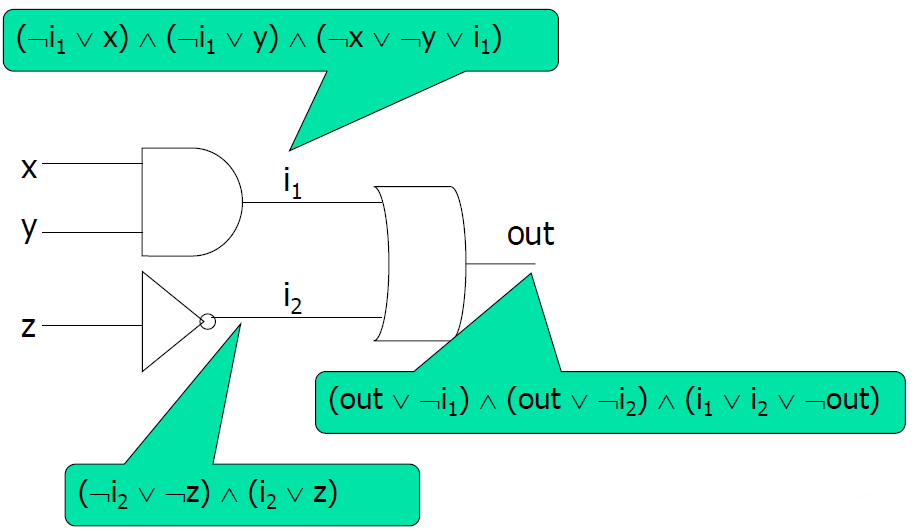
\includegraphics[scale =0.5]{tseitin1.png}
      \caption{Tseitin transformation of a circuit to $CNF$.}
	  \label{fig:tss2}
      \end{center}
      \end{figure}
\end{examp}
%--------------------------------------------------------------------------------------------------------------------------------------
\section{Binary Decision Diagram}
\label{sec:Binary Decision Diagram}

\begin{defi}\label{def:bdd} 
      \textbf{A Binary Decision Diagram (BDD)} is a data structure that is used to represent a boolean function. 
      On a more abstract level, BDDs can be considered as a compressed representation of sets or relations. 
      The basic idea from which the data structure was created is the \href{https://en.wikipedia.org/wiki/Boole%27s_expansion_theorem}{Shannon expansion}. 
	  A switching function is split into two sub-functions (cofactors) by assigning one variable. 
\end{defi} 
\begin{examp}\label{exp:bdd}
      As an BDD, consider the boolean function $f(v_1,v_2,v_3) := v_1 \implies (v_2 \iff v_3)$, with the truth table given in Fig \ref{fig:BooleanFunctionDTExampTT}, 
	  may be represented by either of the BDD shown in Fig \ref{fig:BooleanFunctionDTExampDT1} or Fig \ref{fig:BooleanFunctionDTExampDT2}. 
      $$f(v_1,v_2,v_3) = \{ \{ \overline{v_1},\overline{v_2}, v_3 \}, \{ \overline{v_1}, v_2, \overline{v_3}\} \}$$
      \begin{figure}[h]
            \centering
            \begin{tabular}{|c|c|c|c|} 
                  \hline
                  $v_1$ & $v_2$ & $v_3$ & $v_1 \implies (v_2 \iff v_3)$ \\ \hline
                  0 & 0 & 0 & 1 \\ \hline
                  0 & 0 & 1 & 1 \\ \hline
                  0 & 1 & 0 & 1 \\ \hline
                  0 & 1 & 1 & 1 \\ \hline
                  1 & 0 & 0 & 1 \\ \hline
                  1 & 0 & 1 & 0 \\ \hline
                  1 & 1 & 0 & 0 \\ \hline
                  1 & 1 & 1 & 1 \\ \hline
            \end{tabular}
            \caption{Truth table for boolean function $f$.}
            \label{fig:BooleanFunctionDTExampTT}
      \end{figure}
      \begin{figure}[h]
            \centering
            \begin{displaymath}
                  \xygraph{
                  []{v_1} ( 
                  - [dll]{1}_0 (),
                  - [drr]{v_2}^1 (
                  - [dll]{v_3}_0 (
                  - [dl]{1}_0 (),
                  - [dr]{0}^1 ()
                  ),
                  -[drr]{v_3}^1 (
                  - [dl]{0}_0 (),
                  - [dr]{1}^1 ()
                  )
                  )
                  )
                  }
            \end{displaymath}
            \caption{A BDD representation of $f$.}
            \label{fig:BooleanFunctionDTExampDT1}
      \end{figure}
      \begin{figure}[h]
            \centering
            \begin{displaymath}
                  \xygraph{
                 []{v_2} ( 
                 - [dlll]{v_3}_0 (
                 - [dl]{1}_0 (),
                 - [dr]{v_1}^1 (
                 - [dl]{1}_0 (),
                 - [dr]{0}_1 ()
                 )
                 ),
                 - [drrr]{v_3}^1 (
                 - [dl]{v_1}_0 (
                 - [dl]{1}_0 (),
                 - [dr]{0}^1 ()
                 ),
                 -[dr]{1}^1 ()
                 )
                 )
                 }
            \end{displaymath}
           \caption{Another BDD representation of $f$.}
           \label{fig:BooleanFunctionDTExampDT2}
      \end{figure}
\end{examp}
%--------------------------------------------------------------------------------------------------------------------------------------
%--------------------------------------------------------------------------------------------------------------------------------------
\section{The SAT Problem}
\label{sec:The SAT Problem}

\begin{defi}\label{def:sat} Basically, the meaning of \textbf{the SAT problem} is that for a conjunctive normal form $F$, decide whether $F$ is satisfiable or not.
      The SAT problem is one of the most versatile NP-complete problems. On the theoretical side, due to its expressiveness and flexibility it 
      serves as a tool for many results in complexity theory. On the practical side, NP-completeness of SAT is used “positively”, and many problems 
      are translated into  the “universal language” SAT and solved via SAT solvers. 
\end{defi}

%--------------------------------------------------------------------------------------------------------------------------------------
\section{Backtracking for SAT}
\label{sec:Backtracking for SAT}

\begin{defi}\label{def:bsat} \textbf{Backtracking} is a general algorithm for finding all (or some) solutions to constraint satisfaction problems, 
      that incrementally builds candidates to the solutions, and abandons each partial candidate $c$ ("backtracks") as soon as it determines that c cannot 
      possibly be completed to a valid solution. 

      In general, a backtracking solver can be described as the following recursive procedure on input $F$:
      \begin{enumerate}
            \item First we try to simplify $F$ (using for example unit clause elimination as often as we can).
            \item Then, using simple criterions, we check whether we immediately see, whether $F$ is satisfiable or
            unsatisfiable, in which case we return "satisfiable" resp. "unsatisfiable".
            \item Otherwise some "branching variable" v in $F$ is chosen, and it is determined which truth value $\epsilon \in \{ 0, 1\}$ to consider first.
            \item Compute $\langle v \to \epsilon \rangle * F$, the result of setting variable v to value $\epsilon$, and apply the procedure recursively to
            $\langle v \to \epsilon \rangle * F$. If the result is "satisfiable" then we return "satisfiable".
            \item Otherwise, the second branch $\langle v \to \overline{\epsilon} \rangle * F$ has to be considered: If the result is “satisfiable” then
            “satisfiable” is returned, otherwise “unsatisfiable”.
      \end{enumerate}
\end{defi}
\begin{examp}\label{exp:bdd}
      If the number of variables in CNF $F$ is $n$, then we have $2^n$ assignments in order to find out whether $F$ is satisfiable or not.
      If $n$ is a large number, it would be very difficult to consider all the assignments and we need something more clever.
      The basic idea is to make case distinctions on variables, and to exploit simplifications enabled by these case distinctions.
      Here, we explain this idea using a simple example. Consider the $F = \{ \{c,b\}, \{\overline{c},b,a\}, \{\overline{b},c\}, \{\overline{b},c,a\}, \{{\overline{a},b}\} \}$. 
      %We have 3 variables and $2^3 = 8$ assignments in order to find out whether $F$ is satisfiable or not. If the number of variables is larger, 
      For the first case distinction, we consider $\langle a \to 0 \rangle$:
      $$ F_1 := \langle a \to 0 \rangle * F = \{ \{c,b\}, \{\overline{c},b\}, \{\overline{b},c\}, \{\overline{b},c\} \}$$
      Then, we split on $b$ and:
      $$ F_2 := \langle b \to 0 \rangle * F = \{ \{c\}, \{\overline{c}\} \}$$
      which is $\Usat$. So, we have to backtrack to the last case and consider $\langle b \to 1 \rangle$. We have:
      $$ F_3 := \langle b \to 1 \rangle * F = \{ \{c\}, \{\overline{c}\} \}$$
      which is again $\Usat$. So, we have to backtrack to the higher level, that is, we have to consider $\langle a \to 1 \rangle$:
      $$ F_4 := \langle a \to 1 * F = \{ \{b\} \}.$$
      And  now, if we consider $\langle b \to 1 \rangle$ the result is $\Sat$. It is obvious that this example was simple. But, if we have more variables, 
      sometimes we need to backtrack to the 2-higher level or more to investigate the satisfiablity of $F$.
\end{examp}
%--------------------------------------------------------------------------------------------------------------------------------------
\section{Methods to Address SAT}
\label{sec:Methods to Address SAT}

?????????????\\
Complete (systematic) Methods: DP, DPLL\\
-Explore the space of all possible assignments systematically \\
-If there is a satisfying assignment, it will be found \\
-If no satisfying assignment is found, the formula is unsatisfiable \\

Incomplete (Stochastic) Methods: GSAT, WALKSAT\\
-Stochastic moves in the space of all possible assignments\\
-If there is a satisfying assignment, it may be found\\
-If no satisfying assignment is found, the formula may or may not be unsatisfiable\\
%***************************************************************************************************************************************************************
%***************************************************************************************************************************************************************
\chapter{Hardness Measures}
\label{cha:Hardness Measures}

\section{Implication-relation}
\label{sec:Implication-relation}

\begin{defi}\label{def:models}
  For $F, G \in \Cls$ holds \bmm{F \models G} if $\fa\, \vp \in \Pass : \vp * F = \top \Ra \vp * G = \top$. For $C \in \Cl$ we write \bmm{F \models C} if $F \models \set{C}$.
\end{defi}
Remarks:
\begin{enumerate}
\item $F \in \Usat$ iff $F \models \bot$.
\item If $F \models C$ and $C \sse C'$, then $F \models C'$.
\item The logical-implication-relation (or ``entailment relation'') is a quasi-order on $\Cls$ (is reflexive and transitive).
\item $F \models C$ iff $C * F \in \Usat$.
\item $F \models G$ iff $\fa\, D \in G : F \models D$ iff $\fa\, D \in G : D * F \in \Usat$.
\end{enumerate}

\begin{defi}\label{def:primec}
  An \textbf{implicate} of $F \in \Cls$ is a clause $C \in \Cl$ with $C* F \in \Usat$ (a falsifying assignment, as a partial assignment), while a \textbf{prime implicate} is a minimal implicate (regarding the subset-relation); the set of all prime implicates is denoted by $\bmm{\primec_0(F)} \in \Cls$.

  An \textbf{implicant} of $F \in \Cls$ is a clause $C \in \Cl$ with $C * F = \top$ (a satisfying assignment, as a partial assignment), while a \textbf{prime implicant} is a minimal implicant; the set of all prime implicants is denoted by $\bmm{\primec_1(F)} \in \Cls$.
\end{defi}
Remarks:
\begin{enumerate}
\item A clause $C \in \Cl$ is an implicate of $F \in \Cls$ iff $F \models C$.
\item While $C$ is an implicant of $F$ iff $\set{\set{x} :x \in C} \models F$.
\item $F \in \Usat$ iff $\primec_0(F) = \set{\bot}$, and $F \in \Sat$ iff $\bot \notin \primec_0(F)$.
\item $F \in \Sat$ iff $\primec_1(F) \ne \top$, and $F \in \Usat$ iff $\primec_1(F) = \top$.
\item $\primec_0(\primec_0(F)) = \primec_0(F) = \primec_1(\primec_1(F))$.
\item $\primec_1(\primec_0(F)) = \primec_1(F) = \primec_0(\primec_1(F))$.
\end{enumerate}

\begin{examp}\label{exp:aaa}
      For $F = \{ \{a\}, \{ \overline a, b \}, \{ \overline a, \overline b, c \} \}$ we have:
      $$ prc_0(F) = \{ \{a\}, \{ b \}, \{ c \} \} $$
\end{examp}

\begin{examp}\label{exp:imp3}
      For the boolean function $ a \vee b$ we have $prc_0(a \vee b) = \{ \{a, b \} \}$, while for the boolean function 
	  $a \wedge b$ we have $prc_0(a \wedge b) = \{ \{ a \}, \{b\}\}$.
\end{examp}

\begin{examp}\label{exp:bbb}
      Here, some of other examples are presented:
	  \begin{enumerate}
	        \item For $F = \{\{x, y\} , \{x,\neg y\}\}, prc_0(F) = \{\{x\}\}$.
			\item For $F = \{\{ \neg x, y\} , \{ \neg y, z\}\}, prc_0(F) = \{\{\neg x, y\} , \{\neg y, z\} , \{\neg x, z\}\}$.
			\item For $F = \{\{z, x, y\} , \{z, x, \neg y\} , \{z, \neg x, y\} , \{z,\neg x, \neg y\}\}, prc_0(F) = \{\{z\}\}.$.
      \end{enumerate}
\end{examp}

\begin{defi}\label{def:logequiv}
  Clause-sets $F, G \in \Cls$ are \textbf{logically equivalent} if $F \models G$ and $G \models F$.
\end{defi}
Remarks:
\begin{enumerate}
\item Logical equivalence is an equivalence relation on $\Cls$.
\item $\primec_0(F)$ is logically equivalent to $F$.
\end{enumerate}

\begin{lem}\label{lem:logequiv}
  For $F, G \in \Cls$ the following properties are equivalent:
  \begin{enumerate}
  \item $F, G$ are logically equivalent.
  \item $\primec_0(F) = \primec_0(G)$.
  \item $\primec_1(F) = \primec_1(G)$.
  \end{enumerate}
\end{lem}

\begin{defi}\label{def:forced1}
      A literal $x$ is \textbf{forced} for a boolean function $F$ if $F \models x$.
\end{defi}
\begin{defi}\label{def:imp3}
      A boolean function $f$ is \textbf{monotone} iff flipping any input variable from 0 to 1 never flips the output from 1 to 0.
	  A boolean function $f$(or its corresponding CNF-clause-set $F$) is monotone iff f has only positive prime implicates \cite{h8}.
\end{defi}
%--------------------------------------------------------------------------------------------------------------------------------------
\section{Resolution}
\label{sec:Resolution}

\begin{defi}\label{def:Resolution}
 Two clauses $C,D$ are \textbf{resolvable} if $\abs{C \cap \overline D} = 1$ , i.e., they clash in exactly one variable:
\begin{itemize}
 \item For two resolvable clauses $C$ and $D$ the \textbf{resolvent} $C \diamond D := (C \cup D) \setminus \{x, \overline x\} $ for $C \cap \overline D = \{ x \}$ 
 is the union of the two clauses minus the resolution literals.
 \item x is called the \textbf{resolution literal}, while var(x) is the \textbf{resolution variable} \cite{h5}.
 \end{itemize}
 \end{defi}
 
 Remarks:
\begin{enumerate}
\item The closure of $F \in \Cls$ under resolution is a clause-set with $\primec_0(F)$ as its subsumption-minimal elements.
\item For $F \in \Pcls{2}$ the closure of $F$ under resolution is in $\Pcls{2}$ \cite{h5}.
\end{enumerate}

\begin{examp}\label{exp:resolution1}
       For $C,D,X,Y \in \Cl$, let $C=\{a,b, \neg c\}$ and $D=\{\neg a, \neg d\}$. The resolvent of $C,D$ is $\{b, \neg c, \neg d\}$.
	   But for $X=\{a,b, \neg c\}$ and $Y=\{\neg a, \neg b, d\}$, they are nor resolvable since $\abs{X \cap \overline Y } \not = 1$.
\end{examp}
%--------------------------------------------------------------------------------------------------------------------------------------
\section{Trees}
\label{sec:Trees}

The definition of resolution trees are presented in section \ref{sec:Resolution-tree} but they are closely related to "splitting" or "brancing" trees , full binary trees labelled with clause-sets and corresponding 
to the backtracking tree of the simplest recursive SAT solver on unsatisfiable inputs. It seems that this connection breaks when it comes 
to full resolution, but this is actually only partially so: regarding the number of different clauses in a resolution tree, it is known 
that regularisation can indeed exponentially increase the number of different clauses, however when it comes to width, symmetric or 
asymmetric, then there are no difficulties, since the process of regularisation, implicit in the correspondences between resolution
trees and branching trees, does never increase clause-sizes.
Formally, the branching trees for a clause-set $F \in \Usat$ are the full binary trees obtained as follows:
\begin{enumerate}
\item If $\bot \in F$, then only branching tree for F is the one-node tree labelled with $F$.
\item Otherwise, the branching trees for $F$ are obtained by choosing a variable $v \in \Va$, labelling the root with $F$, and choosing 
a branching tree for $\langle v \rightarrow 0 \rangle * F$ as left subtree and a branching tree for $\langle v \rightarrow 1 \rangle * F$ as right subtree \cite{h5}.
\end{enumerate}

%"Binary Decision Diagram"mentioned in definition \ref{def:bdd}
%--------------------------------------------------------------------------------------------------------------------------------------
\section{Resolution-tree}
\label{sec:Resolution-tree}

\begin{defi}\label{def:restree}
  A \textbf{resolution tree} is a pair $(T,C)$ with:
  \begin{itemize}
  \item $T$ is an ordered rooted tree, where every inner node has exactly two children, and where the set of nodes is denoted 
  by $\nds(T)$, the root by $\rt(T) \in \nds(T)$, and the set of leaves by $\lvs(T) \sse \nds(T)$.
  \item While $C: \nds(T) \ra \Cls$ labels every node with a clause such that the label of an inner node is the resolvent of the labels of its two parents.
  \item We use $\bmm{F(T)} := \set{C(w) : w \in \lvs(T)}$ for the ``axioms'' (or ``premisses'') of $T$ and $\bmm{C(T)} := C(\rt(T))$ as the ``conclusion'' \cite{h5}.
  \end{itemize}
\end{defi}
\begin{defi}\label{def:resproof}
  A \textbf{resolution proof} $R$ of a clause $C$ from a clause-set $F$, denoted by \bmm{R: F \vdash C}, is a resolution tree $R = (T,C)$ such that
  \begin{itemize}
  \item $F(T) \sse F$,
  \item $C(T) = C$.
  \end{itemize}
  We use \bmm{F \vdash C} if there exists a resolution proof $R$ of some $C' \sse C$ from $F$ (i.e., $R: F \vdash C'$). 
  \begin{itemize}
  \item The \textbf{tree-resolution complexity} $\bmm{\comptr(R)} \in \NN$ is the number of nodes in $R$, that is, $comptr(R) := \nnds(R) = \abs{\nds(T)}$.
  \item The \textbf{resolution complexity} $\bmm{\compr(R)} \in \NN$ is the number of \emph{distinct} clauses in $R$, that is $\compr(R) := c(F(R))$.
  \end{itemize}
  Finally, for $F \in \Usat$ we set
  \begin{itemize}
  \item $\bmm{\comptr(F)} := \min \set{\comptr(R) \mb R : F \vdash \bot} \in \NN$
  \item $\bmm{\compr(F)} := \min \set{\comptr(R) \mb R : F \vdash \bot} \in \NN$ \cite{h5}.
  \end{itemize}
\end{defi}

 \begin{examp}\label{exp:resproof1}
      Fig \ref{fig:proof1} showes a resolution proof for  $R: F \vdash C$, $C=\{d\}$ and $F = \{\{a,b,c\},\{\neg b,d\},\{\neg a, d\},\{\neg c, d\}\}$. 
	   \begin{figure}
	   \centering  
       \begin{tikzpicture}[grow'=up]				
				\Tree [.${\{d\}}$ [.${\{c,d \}}$ [.${\{a,c,d\}}$ ${\{a,b,c\}}$ ${\{ \neg b,d\}}$ ]
                           [.${\{ \neg a, d\}}$ ] ]
                           [ .${\{ \neg c, d\}}$  ] ]
       \end{tikzpicture}
	   \caption{A resolution proof for eample  \ref{exp:resproof1}.}
	   \label{fig:proof1}
       \end{figure}
\end{examp}

\begin{defi}\label{def:resrefutation}
  A \textbf{resolution refutation} of a clause-set $F$ is a resolution proof deriving $\bot$ from $F$ \cite{h5}. 
\end{defi}
  
Remarks:
\begin{enumerate}
      \item Typically we identify $R$ with $T$, while suppressing $C$.
	  \item Resolution is sound but is incomplete in the sense that it is not guaranteed to derive every clause that is implied by the given $F \in \Cls$. 
	  However, resolution is refutation complete on $\Cls$, i.e., it is guaranteed to derive the empty clause if the given $F$ is unsatisfiable. 
	  This result is the basis for using resolution as a complete algorithm for testing satisfiability: we keep applying resolution until either 
	  the empty clause is derived (unsatisfiable $F$) or until no more applications of resolution are possible (satisfiable $F$) \cite{h6}.
	  \item The number of resolution tree for $F \vdash \bot$ is infinite since we can use any node many times.
\end{enumerate}

 \begin{examp}\label{exp:res1}
      A resolution tree for $F = \{\{a,b\},\{\neg a,b\},\{a, \neg b\},\{\neg a, \neg b\}\}$ is as Fig \ref{fig:resol1}. Since the empty clause 
	  is driven, it is called resolution refutation.
	   \begin{figure}
	   \centering  
       \begin{tikzpicture}[grow'=up]
       \Tree [.$\bot$  [.${\{b\}}$ ${\{a,b\}}$ ${\{\neg a,b\}}$ ]
                           [.${\{ \neg b\}}$ ${\{a, \neg b\}}$ ${\{\neg a, \neg b\}}$ ] ]
       \end{tikzpicture}
	   \caption{A resolution tree for eample  \ref{exp:res1}.}
	   \label{fig:resol1}
       \end{figure}
\end{examp}

\begin{examp}\label{exp:res2}
      A resolution tree for $F = \{\{a\},\{\neg a,b\},\{\neg a, \neg b\}\}$ is as Fig \ref{fig:resol2}. Since the empty clause 
	  is driven, it is called resolution refutation.
	  \begin{figure}[h]
       \centering
       \begin{tikzpicture}[grow'=up]
       \Tree [.$\bot$  [.${\{a\}}$  ]
                           [.${\{ \neg a\}}$ ${\{\neg a, b\}}$ ${\{\neg a, \neg b\}}$ ] ]

       \end{tikzpicture}
	   \caption{A resolution tree for eample  \ref{exp:res2}.}
	   \label{fig:resol2}
       \end{figure}
\end{examp}
 
\begin{examp}\label{exp:res3}
      A resolution tree for $F = \{\{\neg a, \neg b\},\{\neg a,b,\neg c, \neg d\},\{a, \neg d\},\{c, \neg d\}, \{d\}\}$ is as 
	  Fig \ref{fig:resol3}. Since the empty clause is driven, it is called resolution refutation.
	\begin{figure}[h]
    \centering
    \begin{forest}
    for tree={
    grow'=90,
    parent anchor=north,
    child anchor=south,
    math content,
    inner xsep=0pt,
    anchor=west,
    before typesetting nodes={
      if level=0{}{
        if content={}{
          shape=coordinate
        }{
          content/.wrap value={\{#1\}},
        },
      },
    },
    if level=0{
      before drawing tree={x=+.5em},
      for children={
        if n=1{
          calign with current,
          edge path={
            \noexpand\path [draw, \forestoption{edge}] (!u.north west) +(.5em,0) coordinate (a) -- (a |- .child anchor)\forestoption{edge label};
          }
        }{
          edge path={
            \noexpand\path [draw, \forestoption{edge}] (!u.north west) +(.5em,0) -- (.child anchor)\forestoption{edge label};
          }
        },
      }
    }{
      for descendants={
        for parent={
          for children={
            if n=1{
              calign with current,
              edge path={
                \noexpand\path [draw, \forestoption{edge}] (!u.north west) +(1em,0) coordinate (a) -- (a |- .child anchor)\forestoption{edge label};
              }
            }{
              edge path={
                \noexpand\path [draw, \forestoption{edge}] (!u.north west) +(1em,0) -- (.child anchor)\forestoption{edge label};
              }
            },
          }
        }
      }
    },
    if n children=0{tier=terminus}{}
  }
  [\bot, tikz={\draw ([xshift=.5em].north west) -- (q.south);}
    [{\neg a}
      [{\neg a, \neg b}]
      [b
        [{b, \neg c}
          [{b, \neg a, \neg c}, tikz={\draw ([xshift=1em].north west) -- (s.south);}
            [{b, \neg a, \neg c, \neg d}]
          ]
          [a, tier=t, name=q, tikz={\draw ([xshift=1em].north west) -- (s.south);}
            [{a, \neg d}]
          ]
        ]
        [c, tier=t
          [{c, \neg d}]
          [d, name=s]
        ]
      ]
    ]
  ]
  \end{forest}
  \caption{A resolution tree for eample  \ref{exp:res3}.}
  \label{fig:resol3}
  \end{figure}
\end{examp}

\begin{defi}\label{def:regres}
  A resolution tree($(T,C)$ (see Definition \ref{def:resproof}) is \textbf{regular} if along every path from the root to some leaf no resolution variable occurs more than once.
\end{defi}
%--------------------------------------------------------------------------------------------------------------------------------------
\section{Reduction}
\label{sec:Reduction}
\begin{defi}\label{def:red}
   A \textbf{reduction} is a map $r: \Cls \ra \Cls$ such that for all $F, F' \in \Cls$ we have
  \begin{enumerate}
  \item $r(F)$ is satisfiability-equivalent to $F$;
  \item if $\bot \in r(F)$ and for all $C \in F$ there is $C' \in  F'$ with $C' \sse C$, then $\bot \in r(F')$.
  \end{enumerate}
  A reduction $r$ \textbf{discovers} unsatisfiability of $F$ if $\bot \in r(F)$ \cite{h10}.
\end{defi}

\begin{defi}\label{def:implication}
  Consider a reduction $r$. The relation $\bmm{F \models_r C}$ holds for a clause-set $F$ and a clause $C$, and we say \textbf{$C$ is deducible from $F$ via $r$}, if $r$ 
  discovers unsatisfiability of $\vp_C * F$ (that is, $\bot \in r(\vp_C * F)$ for $\vp_C = \pab{x \mapsto 0 : x \in C}$).
\end{defi}

%--------------------------------------------------------------------------------------------------------------------------------------
\section{Generalised unit-clause-propagation}
\label{sec:rkred}

An important special case of resolution is called \textbf{unit resolution (unit propagation)}. Unit resolution is a resolution strategy 
which requires that at least one of the resolved clauses has only one literal. Such clause is call a \textbf{unit clause}. Unit resolution 
is not refutation complete, which means that it may not derive the empty clause from an unsatisfiable $CNF$ formula. Yet one can apply all 
possible unit resolution steps in time linear in the size of given CNF. Because of its efficiency, unit resolution is a key technique 
employed by a number of algorithms \cite{h6}.

The unit resolution technique (or unit propagation) is quite simple: first, we close the CNF under unit resolution and collect all unit 
clauses in the $CNF$. We then assume that variables are set to satisfy these unit clauses. That is, if the unit clause $\{x\}$ appears 
in the $CNF$, we set $x$ to true. And if the unit clause $\{\neg x\}$ appears in the $CNF$, we set $x$ to false. We then simplify the 
$CNF$ given these settings and check for either success (all clauses are subsumed) or failure (the empty clause is derived)\cite{h6}.

\begin{examp}\label{exp:unit1}
      Let $F=\{ \{a\}, \{a, b\}, \{\neg a, c\}, \{\neg c, d\}\}$. By unit propagation (because $F$ contains the unit clause $\{a\}$), 
	  we obtain $\varphi_a * F=\langle a \rightarrow 1 \rangle * F= \{ \{c\}, \{\neg c, d\}\}$. If $\bot \in \varphi_a * F$, then $F$ is 
	  satisfiability-equivalent to $\varphi_a * F$ and we eliminated one variable. Otherwise, we know that all clauses in $\varphi_a * F$ 
	  must have length at least 2. So, in this case $F$ is also satisfiability equivalent to $\varphi_a * F$, and again at least one 
	  variable has been eliminated.
\end{examp}

\begin{defi}\label{def:rk}
  The maps $\bmm{\rk_k}: \Cls \ra \Cls$ for $k \in \NNZ$ are defined as follows (for $F \in \Cls$):
  \begin{eqnarray*}
    \rk_0(F) & := &
    \begin{cases}
      \set{\bot} & \text{if } \bot \in F\\
      F & \text{otherwise}
    \end{cases}\\
    \rk_{k+1}(F) & := &
    \begin{cases}
      \rk_{k+1}(\pao x1 * F) & \text{if } \ex\, x \in \lit(F) : \rk_k(\pao x0 * F) = \set{\bot}\\
      F & \text{otherwise}
    \end{cases}.
  \end{eqnarray*}
\end{defi}
Remarks:
\begin{enumerate}
\item $\rk_1$ is unit-clause propagation, $\rk_2$ is (full) failed literal elimination.
\item In general we can call $\rk_k$ \textbf{$k$-propagation-reduction} or \textbf{generalised unit-clause-propagation of level $k$}.
\end{enumerate}

\begin{examp}\label{exp:rk}
  Computing some $\rk_k(F)$, using literals $x,y,x_1,\dots,x_n$ ($n \in \NNZ$) with distinct underlying variables:
  \begin{enumerate}
  \item $\rk_k(\set{\bot}) = \set{\bot}$ for $k \ge 0$.
  \item $\rk_k(\top) = \top$ for $k \ge 0$.
  \item For $F := \set{\set{x_1},\dots,\set{x_n}}$: $\rk_0(F) = F$, $\rk_k(F) = \top$ for $k \ge 1$.
  \item For $F' := F \cup \set{\set{x,y}}$: $\rk_0(F') = F'$, $\rk_k(F') = \set{\set{x,y}}$ for $k \ge 1$ (note that $\set{\set{x,y}}$ has no forced assignments).
  \item For $F := \set{\set{x,y},\set{x,\ol{y}}}$: $\rk_k(F) = F$ for $k \le 1$, $\rk_k(F) = \top$ for $k \ge 2$.
  \item For $F := \set{\set{x,y},\set{x,\ol{y}}, \set{\ol{x},y},\set{\ol{x},\ol{y}}}$: $\rk_k(F) = F$ for $k \le 1$, $\rk_k(F) = \set{\bot}$ for $k \ge 2$.
  \end{enumerate}
\end{examp}

%--------------------------------------------------------------------------------------------------------------------------------------
\section{Horton-Strahler Number}
\label{sec:hs}
\begin{defi}\label{def:hdtree}
  Consider a resolution tree $T$ (recall Definition \ref{def:resproof}). The \textbf{Horton-Strahler} number $\bmm{\hts(T)} \in \NNZ$ is defined as $\hts(T) := 0$, if $T$ is trivial (consists only of one node), while otherwise we have two subtrees $T_1, T_2$, and we set $\hts(T) := \max(\hts(T_1),\hts(T_2))$ if $\hts(T_1) \not= \hts(T_2)$, while in case of $\hts(T_1) = \hts(T_2)$ we set $\hts(T) := \max(\hts(T_1),\hts(T_2)) + 1$.
\end{defi}

\begin{examp}\label{exp:hortonstrahler}
  Fig \ref{fig:hst} showes some examples of trees with their Horton-Strahler numbers. We denote by $T_1$ and $T_2$ in each example the left and right sub-trees of the root.
 \begin{figure}[h] 
  \begin{center}
  %\centring
    \begin{tabular}{|>{\centering\arraybackslash}m{10em}|>{\centering\arraybackslash}m{3em}|>{\centering\arraybackslash}m{7em}|}
      \hline
      \textbf{Tree $T$} & \bmm{\hts(T)} & \textbf{Explanation} \\\hline\hline
      $\displaystyle
      \xygraph{
        []{\cdot} ( )
      }$ & 0 & trivial tree \\ \hline
      $\displaystyle
      \xygraph{
        !{0;/r3ex/:}
        []{\cdot} (
          - [dl]{\cdot} (),
          - [dr]{\cdot} ()
        )
      }$ & 1 & $\hts(T_1) = 0$, $\hts(T_2) = 0$. \\ \hline
      $\xygraph{
        !{0;/r3ex/:}
        []{\cdot} (
        - [dl]{\cdot} (),
        - [dr]{\cdot} (
          -[dl]{\cdot} (),
          -[dr]{\cdot} ()
        )
        )
      }$ & 1 & $\hts(T_1) = 0$, $\hts(T_2) = 1$.  \\ \hline
      $\xygraph{
        !{0;/r3ex/:}
        []{\cdot} (
          - [dl]{\cdot} (),
          - [dr]{\cdot} (
            -[dl]{\cdot} (),
            - [dr]{\cdot} (
              -[dl]{\cdot} (),
              -[dr]{\cdot} ()
            )
          )
        )
      }$ & 1 & $\hts(T_1) = 0$, $\hts(T_2) = 1$.  \\ \hline
      $\xygraph{
        !{0;/r3ex/:}
        []{\cdot} (
        - [dll]{\cdot} (
          -[dl]{\cdot} (),
          -[dr]{\cdot} ()
        ),
        - [drr]{\cdot} (
          -[dl]{\cdot} (),
          -[dr]{\cdot} ()
        )
        )
      }$ & 2 & $\hts(T_1) = 1$, $\hts(T_2) = 1$.  \\ \hline
      $\xygraph{
        !{0;/r3ex/:}
        []{\cdot} (
        - [dll]{\cdot} (
          -[dl]{\cdot} (),
          -[dr]{\cdot} ()
        ),
        - [drr]{\cdot} (
          -[dll]{\cdot} (
            -[dl]{\cdot} (),
            -[dr]{\cdot} ()
          ),
          -[dr]{\cdot} (
            -[dl]{\cdot} (),
            -[dr]{\cdot} ()
          )
        )
        )
      }$ & 2 & $\hts(T_1) = 1$, $\hts(T_2) = 2$.  \\ \hline
    \end{tabular}
  \end{center}
  \caption{Horton-Strahler numbers of some trees.}
  \label{fig:hst}
  \end{figure}
\end{examp}

\begin{defi}\label{def:geninpres}
      For a clause-set $F$ and a clause $C$ the relation \bmm{F \vdash_k C} ($C$ can be derived from $F$ by \textbf{$k$-times nested input resolution}) if there exists a resolution tree $T$ and $C' \sse C$ with $T : F \vdash C'$ and $\hts(T) \le k$.
\end{defi}
%--------------------------------------------------------------------------------------------------------------------------------------
\section{Hardness}
\label{sec:Hardness}
%--------------------------------------------------------------------------------------------------------------------------------------
\subsection{Hardness of Unsatisfiable Clause-sets}
\label{sec:Hardnessunsat}
Hardness $\hardness :\Cls \rightarrow \NNZ$ is a measure for SAT representation "complexity". The basic idea is to start with some measurement
$ h : \Usat \rightarrow \NNZ$ of the complexity of unsatisfiable $F$. This measure is extended to arbitrary $F \in \Cls$ by maximising 
over all "sub-instances" of $F$, that is, over all unsatisfiable $\varphi * F$ for (arbitrary) partial assignments $\varphi$.

However, there are various equivalent descriptions for hardness. It seems that this concept was reinvented in the literature several times. 
Intuitively, the hardness measures the height of the biggest full binary tree which can be embedded into each tree-like resolution 
refutation of the formula. This is also known as the Horton-Strahler number of a tree. There is another equivalent description, 
which uses generalised unit-clause propagation $r_k$ to measue hardness. Following, these two description are presented.

\begin{defi}\label{def:hardness1}
      For $F \in \Usat$ let \textbf{hardness} $\bmm{\hardness(F)} \in \NNZ$ be the minimal $k \in \NNZ$ such that a resolution tree $T : F \vdash \bot$ 
	  exists, where the Horton-Strahler number of $T$ is at most $k$. For $k \in \NNZ$ let $\Urefc_k  := \{F \in \Cls : \hardness(F) \leq k\}$ \cite{h5}.
\end{defi}
And according to \cite{h13}:
\begin{defi}\label{def:hardness2}
  The \textbf{hardness} $\hardness(F)$ of an unsatisfiable $F \in \Cls$ is the minimal $k \in \NNZ$ such that $\rk_k(F) = \set{\bot}$.
\end{defi}

\begin{examp}\label{exp:hardness1}
      For $\set{\set{x,y},\set{x,\ol{y}},\set{\ol{x},y},\set{\ol{x},\ol{y}}}$ we have $r_1(F)=F, r_2(F)=r_2( \langle a \rightarrow 1 \rangle * F) = \{ \bot \}$
	  (since $r_1( \langle a \rightarrow 0 \rangle * F)=r_1 (\{\{ b \}, \{ \neg b \}\}) = \{ \bot \}$). Thus, $\hardness(F) = 2$.
\end{examp}

\begin{examp}\label{exp:harducls}
  Here are some basic determinations of $\hardness(F)$ for unsatisfiable clause-sets $F$, using literals $x,y,z$ with distinct underlying variables:
  \begin{enumerate}
  \item $\hardness(F) = 0$ iff $\bot \in F$.
  \item $\hardness(\set{\set{x},\set{\ol{x}}}) = 1$.
  \item $\hardness(\set{\set{x},\set{\ol{x},y}, \set{\ol{y},z}, \set{\ol{z}}}) = 1$.
  \item $\hardness(\set{\set{x,\ol{y}},\set{\ol{x},y},\set{y,\ol{z}},\set{\ol{y},z},\set{x,y,z},\set{\ol{x},\ol{y},\ol{z}}}) = 2$.
  \end{enumerate}
\end{examp}

\begin{defi}\label{def:hardness2}
      For $F \in \Usat$ let $\textbf{dep(F)} \in \NN_0$ be the minimal height of a resolution tree $T : F \vdash \bot$.
\end{defi}

Remarks:
\begin{enumerate}
  \item Since the Horton-Strahler number of a tree is at most the height, we get $\hardness(F) \leq dep(F)$ for all $F \in \Cls$.
\end{enumerate}
%--------------------------------------------------------------------------------------------------------------------------------------
\subsection{Extension of hardness to satisfiable clause-sets}
\label{sec:extension_Hardness}

It is important to extend measures of hardness for unsatisfiable clause-set to arbitrary clause-set(both satisfiable and unsatisfiable).????
\begin{defi}\label{def:ex-hardness}
The hardness $\hardness : \Cls \rightarrow \NNZ$ is defined for $F \in \Cls$ as follows:
\begin{enumerate}
  \item If $F \in \Usat$ , then $\hardness(F)$ is the minimum hs(T ) for $T : F \vdash \bot$.
  \item If $F = \top$, then $\hardness(F) := 0$.
  \item If $F \in \Sat \ \{ \top \}$, then $\hardness(F) := \max \{ \hardness(\varphi * F) : \varphi * F \in \Usat \}$ \cite{h11}.
  \end{enumerate}
\end{defi}
%--------------------------------------------------------------------------------------------------------------------------------------
\section{Width-hardness}
\label{sec:whd}
%--------------------------------------------------------------------------------------------------------------------------------------
\subsection{Width-hardness of Unsatisfiable Clause-sets}
\label{sec:whdd}

The standard resolution-width of an unsatisfiable clause-set $F$ is the minimal $k$ such that a resolution refutation of $F$ using only 
clauses of length at most $k$ exists \cite{h5}.

\begin{defi}\label{def:whd1}
     For  $F \in \Usat$ the \textbf{symmetric width} $\bmm{\wid(F)} $\in \NNZ$ is the smallest $k \in \NNZ$ such that there is
	 $T : F \vdash \bot$ with $\widehat{F}(T) \in k-\Cls$.
\end{defi}
\begin{defi}\label{def:whd}
  For a resolution tree $T$ its \textbf{(asymmetric) width} $\bmm{\whardness(T)} \in \NNZ$ is defined as $0$ if $T$ is trivial (i.e., $\abs{\nds(T)} = 1$), while otherwise for left and right children $w_1, w_2$ with subtrees $T_1, T_2$ we define
  \begin{displaymath}
    \whardness(T) := \max \big (\whardness(T_1), \whardness(T_2), \, \min(\abs{C(w_1)}, \abs{C(w_2)}) \big )
  \end{displaymath}
  (note that the corresponding definition of $\wid(T)$ just has the $\min$ replaced by a (second) $\max$). We write \bmm{R : F \vdash^k C} if $R : F \vdash C$ and $\whardness(R) \le k$. Now for $F \in \Usat$ we define $\bmm{\whardness(F)} := \min \set{\whardness(T) \mb T : F \vdash \bot}\in \NNZ$. For $k \in \NNZ$ let $\bmm{\Wrefc_k} := \set{F \in \Cls : \whardness(F) \le k}$.
\end{defi}
Remarks:
	    \begin{enumerate}
              \item For all $F \in \Cls $ holds \whardness(F)$ \leq \hardness(F)$.
		\end{enumerate}
\begin{examp}\label{exp:whd1}
      Some examples for $\wid(F)$ and $\whardness(F)$ are as below:
	    \begin{enumerate}
              \item $\wid(\set{\bot}) = \whardness(\set{\bot}) = 0$.
			  \item More generally for $C \in \Cl$ holds $wid(\{C\}) = \whardness(\{C\}) = 0$.
			  \item In general we have $\wid(F) = 0 \Leftrightarrow \whardness(F) = 0$ for all $F \in \Cls$.
			  \item For a Horn clause-set $F$ holds $\whardness(F) \leq 1$ (since unit-clause propagation is sufficient to derive unsatisfiability), 
			  while $\wid(F)$ is unbounded (if $F$ is minimally unsatisfiable, then $\wid(F)$ equals the maximal clause-length of $F$).
			  \item For general minimally unsatisfiable $F$, the maximal clause-length is a lower bound for $\wid(F)$, but is unrelated to 
			  $\whardness(F)$.
      	\end{enumerate}		  
\end{examp}

\begin{examp}\label{exp:whd2}
      For $F := \{\{a\}, \{a, b\}, \{a, b\}\}$ there are two possible trees as $T_1$ in Fig \ref{fig:whd2} and $T_2$ in Fig \ref{fig:resol2}.   
	  Using definition \ref{def:whd2}, we have $\whardness(T_1) = 1$ and $\whardness(T_2) = 2$ and finally $\whardness(F) = 1$. $\wid(F) = 2$ is also 
	  obtained by definition \ref{def:whd1}.
	  \begin{figure}
      \begin{center}
	  %\centering
      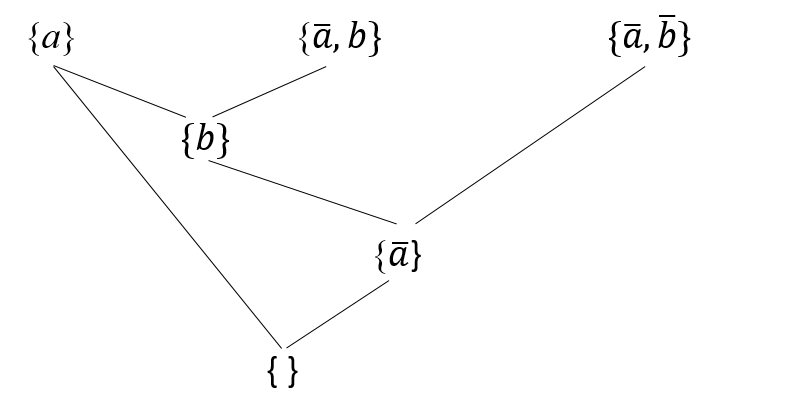
\includegraphics[scale =0.6]{whd1.png}
      \caption{The esolution tree $T_1$ in \ref{exp:whd2}.}
	  \label{fig:whd2}
      \end{center}
      \end{figure}
\end{examp}

%--------------------------------------------------------------------------------------------------------------------------------------
\subsection{The relation between symmetric and asymmetric width}
\label{sec:The relation between wid awid}


%--------------------------------------------------------------------------------------------------------------------------------------
\subsection{Extension of Width-hardness to satisfiable clause-sets}
\label{sec:extensionWidth-hardness}

\begin{defi}\label{def:ex-whd}  
      The \textbf{width-hardness} $\whardness : \Cls \rightarrow \NNZ$  is defined for $F \in \Cls$ as follows:
	  \begin{enumerate}
              \item If $F \in \Usat$ , then $\whardness(F)$ is the minimum $k \in \NNZ$ such that k-resolution refutes $F$, that is, such that
			  $T : F \vdash \bot$ exists where for each resolution step $R = C  \diamond D$ in $T$ we have $ \abs{C } \leq k$ or $\abs{D } \leq k$.
			  \item If $F = \top$, then $\whardness(F) := 0$.
			  \item If $F \in \Sat \ \{ \top \}$, then $\whardness(F) := \max \{\whardness(\varphi * F) : \varphi * F \in \Usat\}$.
      \end{enumerate}
\end{defi}

%--------------------------------------------------------------------------------------------------------------------------------------
\section{Hypergraph}
\label{sec:Hypergraph}

\begin{defi}\label{def:hypergraphs}
  A \textbf{hypergraph} is a pair $G=(V,E)$, where $V$ is a set (the set of ``vertices''), while $E \sse \pote(V)$ is a set of finite subsets of $V$ (the ``hyperedges''). 
  We use for a hypergraph $G = (V,E)$ the notations $\bmm{V(G)} := V$ and $\bmm{E(G)} := E$. A general hypergraph is a triple $(V,E,e)$ where $V, E$ are sets and $e:E \rightarrow \pot_f(V)$ 
  where $\pot_f(V)$ for a set $X$ is the set of finite subsets of $X$: one writes $e(G)=e$ \cite{h5}. 
\end{defi}

\begin{examp}\label{exp:hypergraph1}
      Fig \ref{fig:tss1} showes an example of hypergraph with $V=\{ v_1, v_2, v_3, v_4, v_5, v_6, v_7 \}$ and $E=\{ e_1, e_2, e_3, e_4\} = \{ \{ v_1, v_2, v_3\}, \{v_2, v_3\}, \{ v_3, v_5, v_6\}, \{ v_4 \}\}$.
	   
	\begin{figure}[h]
    \centering  
	\begin{tikzpicture}
    \node (v1) at (0,2) {};
    \node (v2) at (1.5,3) {};
    \node (v3) at (4,2.5) {};
    \node (v4) at (0,0) {};
    \node (v5) at (2,0.5) {};
    \node (v6) at (3.5,0) {};
    \node (v7) at (2.5,-1) {};

    \begin{scope}[fill opacity=0.8]
    \filldraw[fill=yellow!70] ($(v1)+(-0.5,0)$) 
        to[out=90,in=180] ($(v2) + (0,0.5)$) 
        to[out=0,in=90] ($(v3) + (1,0)$)
        to[out=270,in=0] ($(v2) + (1,-0.8)$)
        to[out=180,in=270] ($(v1)+(-0.5,0)$);
    \filldraw[fill=blue!70] ($(v4)+(-0.5,0.2)$)
        to[out=90,in=180] ($(v4)+(0,1)$)
        to[out=0,in=90] ($(v4)+(0.6,0.3)$)
        to[out=270,in=0] ($(v4)+(0,-0.6)$)
        to[out=180,in=270] ($(v4)+(-0.5,0.2)$);
    \filldraw[fill=green!80] ($(v5)+(-0.5,0)$)
        to[out=90,in=225] ($(v3)+(-0.5,-1)$)
        to[out=45,in=270] ($(v3)+(-0.7,0)$)
        to[out=90,in=180] ($(v3)+(0,0.5)$)
        to[out=0,in=90] ($(v3)+(0.7,0)$)
        to[out=270,in=90] ($(v3)+(-0.3,-1.8)$)
        to[out=270,in=90] ($(v6)+(0.5,-0.3)$)
        to[out=270,in=270] ($(v5)+(-0.5,0)$);
    \filldraw[fill=red!70] ($(v2)+(-0.5,-0.2)$) 
        to[out=90,in=180] ($(v2) + (0.2,0.4)$) 
        to[out=0,in=180] ($(v3) + (0,0.3)$)
        to[out=0,in=90] ($(v3) + (0.3,-0.1)$)
        to[out=270,in=0] ($(v3) + (0,-0.3)$)
        to[out=180,in=0] ($(v3) + (-1.3,0)$)
        to[out=180,in=270] ($(v2)+(-0.5,-0.2)$);
    \end{scope}

    \foreach \v in {1,2,...,7} {
        \fill (v\v) circle (0.1);
    }

    \fill (v1) circle (0.1) node [right] {$v_1$};
    \fill (v2) circle (0.1) node [below left] {$v_2$};
    \fill (v3) circle (0.1) node [left] {$v_3$};
    \fill (v4) circle (0.1) node [below] {$v_4$};
    \fill (v5) circle (0.1) node [below right] {$v_5$};
    \fill (v6) circle (0.1) node [below left] {$v_6$};
    \fill (v7) circle (0.1) node [below right] {$v_7$};

    \node at (0.2,2.8) {$e_1$};
    \node at (2.3,3) {$e_2$};
    \node at (3,0.8) {$e_3$};
    \node at (0.1,0.7) {$e_4$};
    \end{tikzpicture}
    \caption{An example of hypergraph.}
    \label{fig:hypergraph1}
    \end{figure}
\end{examp}

%--------------------------------------------------------------------------------------------------------------------------------------
\section{Tseitin Clause-sets}
\label{sec:Tseitin Clause-sets}	  

An "XOR-constraint", or a linear equation over $\ZZ_2$, is a finite set $V \subset \Va$ of variables together with $\ve \in \set{0,1}$, with the 
interpretation $\oplus_{v \in V} v = \ve$. So a \emph{system of XOR-constraints/linear equations} is a pair $(G,\rho)$, where $G$ is a finite 
hypergraph with $V(G) \sse \Va$, and $\rho: E(G) \ra \set{0,1}$ assigns to each hyperedge (an equation) the prescribed sum. The basic associated 
clause-set is $\bmm{X_0(G,\rho)} \in \Cls$ defined as
\begin{displaymath}
  X_0(G,\rho) := X_0(\set{\oplus_{v \in H} = \rho(H)}_{H \in E(G)}) \cite{h5}.
\end{displaymath}

The \textbf{dual} of $(G,\rho)$, written $\trans{(G,\rho)}$, is the pair $(\trans{G}, \rho)$, where
\begin{itemize}
\item $\trans{G}$ is the dual of $G$ as general hypergraph, that is:
  \begin{itemize}
  \item $V(\trans{G}) = E(G)$
  \item $E(\trans{G}) = V(G)$
  \item the hyperedge-function $e: E(\trans{G}) \ra \pote(V(\trans{G}))$ assigns to every $v \in V(G)$ the set of $H \in E(G)$ with $v \in H$;
  \end{itemize}
\item so now $\rho: V(\trans{G}) \ra \set{0,1}$.
\end{itemize}
In general, a \emph{dual system of XOR-constraints/linear equations over $\ZZ_2$} is a pair $(G,\rho)$, where $G$ is a finite general hypergraph 
with $E(G) \sse \Va$ and $\rho: V(G) \ra \set{0,1}$. So the associated system of XOR-constraints is obtained again by dualisation, written again 
$\trans{(G,\rho)} := (\trans{G},\rho)$, where $\trans{G}$ is the dual of $G$ as (ordinary) hypergraph, that is, $V(\trans{G}) = E(G)$ and $E(\trans{G}) = \set{v \in E(G) : w \in e(G)(v)}_{w \in V(G)}$. 
The associated clause-set $\bmm{X_0(G,\rho)} \in \Cls$ is $X_0(G,\rho) := X_0(\trans{(G,\rho)})$.

Obviously dualisation in both directions yields inverse bijections between the set of systems of XOR-constraints and the set of dual systems of XOR-constraints \cite{h5}.

\begin{defi}\label{def:tgraph}
A \textbf{full Tseitin graph} is a dual system of XOR-constraints $(G,\rho)$, where $G$ is a connected irreflexive general graph with 
$\oplus_{w \in V(G)} \rho(w) = 1$, where irreflexive general graphs says $\fa\, v \in E(G) : \abs{e(G)(v)} = 2$. Note that additionally to ordinary (
full) Tseitin graphs we allow parallel edges, but still loops are disallowed (a loop at a vertex in effect deactivates the corresponding equation). 
Now $X_0(G,\rho) \in \Usat$ \cite{h5}.
\end{defi}

An important abstraction is obtained by the insight, that $X_0(G,\rho)$ and $X_0(G,\rho')$ are flipping-isomorphic, that is, by flipping literals we 
can obtain the former from the latter. So we consider plain connected irreflexive general graph with at least one vertex as \textbf{Tseitin graphs}, 
considering implicitly the set of all possible vertex-labellings (with elements from $\set{0,1}$, so that the (XOR-)sum is $1$).

To understand $\hardness(X_0(G))$ and $\whardness(X_0(G))$, we need to understand what splitting does with $G$. The variables $v \in \var(F)$ of 
$F := X_0(G)$ are the edges of $G$:
\begin{itemize}
\item If $G' := G - v$ is still connected, then $\pao v0 * F$ and $\pao v1 * F$ are both isomorphic to $X_0(G')$. Note that $G'$ is still a Tseitin graph.
\item Otherwise let $G', G''$ be the connected components of $G$ (both again Tseitin graphs). Now $\pao v0 * F$ and $\pao v1 * F$ are isomorphic, in some 
order, to $X_0(G'), X_0(G'')$.
\end{itemize}
The endpoint of splitting is reached when $G$ is the one-point graph (which can not have edges, since loops are not allowed) \cite{h5}. 

%--------------------------------------------------------------------------------------------------------------------------------------
\section{Hardness Game}
\label{sec:Hardness Game}	  

???????
The hardness game according to \cite{h5} is as lemma \ref{lem:game1}.
\begin{lem}\label{lem:game1}
      Let $G$ be a Tseitin graph. Then $\hardness(X_0(G))$ is characterised by the following game:
	  \begin{enumerate}
	  \item An atomic move for the current non-trivial Tseitin graph $G$ replaces $G$ with a sub-graph $G'$ of $G$, obtained by choosing 
	  some $e \in E(G)$ and choosing a connected component of $G - e$.
	  \item The two players play in turns, and delayer starts with $G$.
	  \item A move of delayer is to apply a sequence of atomic moves (possibly zero).
	  \item A move of prover is to apply one atomic move.
	  \item The games ends when $G$ becomes trivial, in which case delayer gets as many points as there have been moves by prover.
	  \end{enumerate}
\end{lem}

Remarks:
      \begin{enumerate}
	  \item In hardness game, both delayer and prover have specific types of move which can be categorized (and named) as follows:
	       \begin{enumerate}
		   \item D-A: The graph is symmetric and there is no bridge. So, delayer prefers to take no action.
		   \item D-B: There is a bridge in graph. Delayer removes the bridge and divides the graph into two components. 
		   Then, it chooses the biger component and discards the smaller one.
		   \item D-C: Delayer has to do nothing since if it removes any edge, the game will finish.
		   \item D-D: (In complete graphs) The graph is not symmetric but there is no bridge. If delayer removes any edge, 
		   it might help prover to finish game earlier. Therefore, delayer prefers to take no action.		   
		   \item P-A: The graph is symmetric and prover removes a random edge.
		   \item P-B: There is at least one node with one connected edge. Prover removes the edge and divides the graph into two components: 
		   one isolated node and the rest of graph. Then, it chooses the isolated node and discards the rest of graph and the game finishes.
		   \item P-C: (In complete graphs) The number of connected edges to nodes are not equal and prover chooses the node with smallest
		   connected edges and removes on of them. 
           \end{enumerate}		   
	  \item During the game, if we obtain a complete garph $K_n, n \in \NN$, the hardness would be the sum of prover's points (untill that step) 
	  and $\hardness(K_n).
	  \end{enumerate}
\begin{conj}\label{con:hd_game1}
      For a complete graph $K_n, n \in \NN$, $\hardness(K_n)= (n-1)-1+\hardness(K_{n-1}) $. 
	  
	  Proof: In a complete graph, there are $n-1$ connected edges to each node. 	  Prover chooses a node and removes a connected edge of 
	  that node in each step. Then, when there is only one connected edge to that node(a bridge) delayer removes the bridge and chooses the 
	  $K_{n-1}$ graph. So, $\hardness(K_n)= (n-1)-1+\hardness(K_{n-1}) $.
	  Table \ref{fig:table1} showes $\hardness(K_n)$ for some $n$.
	  \begin{figure}[h]
       \centering
       \begin{tabular}{|c|c|} 
                  \hline
                  $n$ & $\hardness(K_n)$ \\ \hline
                 % 0 & 0  \\ \hline
                  %1 & 0  \\ \hline
				  2 & 1  \\ \hline
				  3 & $1+ \hardness(K_2)=2$ \\ \hline
			      4 & $2+ \hardness(K_3)=4$  \\ \hline
				  5 & $3+ \hardness(K_4)=7$  \\ \hline
				  6 & $4+ \hardness(K_5)=11$  \\ \hline
				  7 & $5+ \hardness(K_6)=16$  \\ \hline
       \end{tabular}
       \caption{The hardness for complete graph $K_n$.}
       \label{fig:table1}
      \end{figure}
\end{conj}

\begin{examp}\label{exp:hd1}
       Fig \ref{fig:game1} showes the atomic moves of hardness game for garph $G1$ (which is called $K_3$) in Fig \ref{fig:hd1}. Delayer starts the game and two 
	   players play in turn. 
	   
	   In first move, the graph is symmetric (no bridge) and delayer chooses to do nothing. Then, prover chooses an edge (in this case, it can remove any edge). 
	   In third move, delayer has to do nothing since removing any edge will lead to ending game. Finally, prover chooses an edge and graph is divided to two components: 
	   one seprate vertex and one edge. So, prover chooses the vertex to finish the game. The hardness of the graph ( which is the number of moves done by prover) is $\hardness(G1)=2$.
	   
	   \begin{figure}[h]
       \centering
       \begin{tabular}{|c|c|} 
                  \hline
                  Delayer & Prover \\ \hline
                  nothing & choosing 1  \\ \hline
                  nothing & choosing 3  \\ \hline
       \end{tabular}
       \caption{The atomic moves for \ref{fig:game1} and \hardness(F)=2.}
       \label{fig:game1}
      \end{figure}
	   %----------------------
	  \begin{figure}
      \begin{center}
	  %\centering
      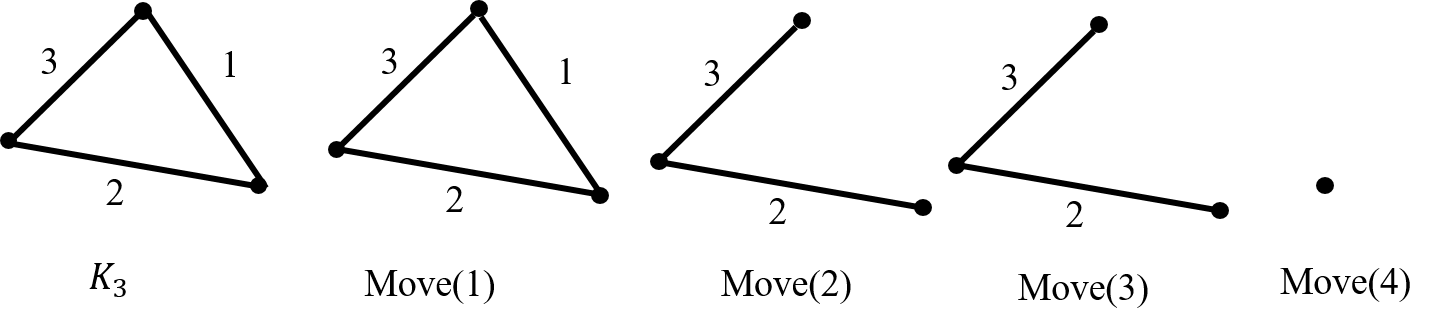
\includegraphics[scale =0.6]{g1.png}
      \caption{The hardness game for G1.}
	  \label{fig:hd1}
      \end{center}
      \end{figure}
\end{examp}

\begin{examp}\label{exp:hd2}
       Fig \ref{fig:game2} showes the atomic moves of hardness game for garph $G2$ in Fig \ref{fig:hd2}. Delayer starts the game and two 
	   players play in turn. 
	   
	   In first move, the graph is symmetric (no bridge) and delayer chooses to do nothing. Then, prover chooses an edge (in this case, it can remove any edge). 
	   In third move, delayer chooses to do nothing since there is no bridge. Then, prover can choose edges 1 or 4 (in this case we continue with removing edge 1) since in each case 
	   the result will be the same. In fifth move, delayer has to remove edge 6 (the bridge) and the graph is devided to two components: 
	   one seprate vertex and the $K_3$ graph. Delayer chooses biger component ( $K_3$ graph) and the rest of the game would be the same as exqample \ref{exp:hd1} and $\hardness(G2)=4$.
	 
	 \begin{figure}[h]
      \centering
      \begin{tabular}{|c|c|} 
      \hline
                  Delayer & Prover \\ \hline
                  nothing & choosing 2  \\ \hline
                  nothing & choosing 1  \\ \hline
                  choosing 6 & choosing 5  \\ \hline
                  nothing & choosing 4 \\ \hline
      \end{tabular}
      \caption{The atomic moves for \ref{fig:game2} and hd(F)=4.}
      \label{fig:game2}
      \end{figure}
	  %---
	  \begin{figure}
      \begin{center}
	  %\centering
      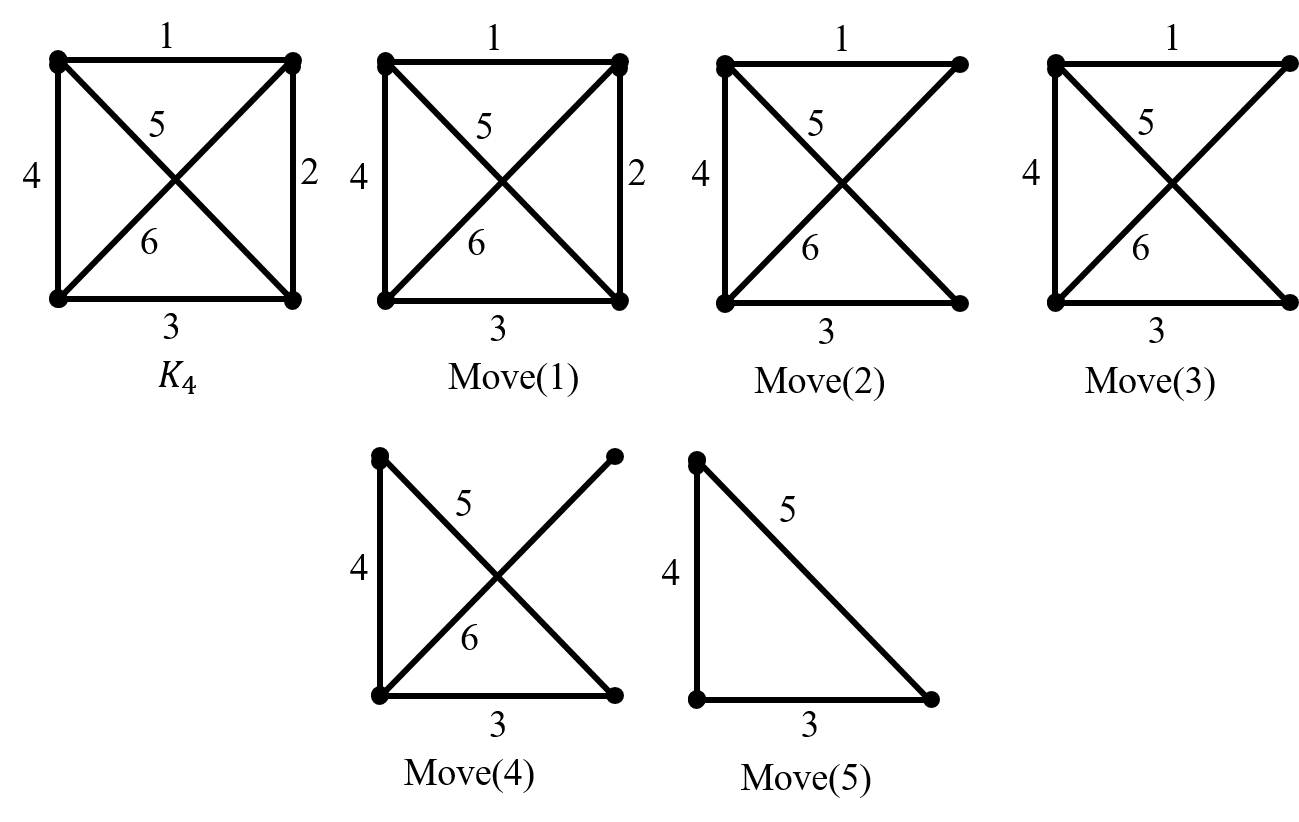
\includegraphics[scale =0.6]{g2.png}
      \caption{The hardness game for G2}
	  \label{fig:hd2}
      \end{center}
      \end{figure}
	   
\end{examp}

\begin{examp}\label{exp:hd3}
       Fig \ref{fig:game3} showes the atomic moves of hardness game for garph $G3$ in Fig \ref{fig:hd3}. Delayer starts the game and two 
	   players play in turn. 
	   
	   In first move, the graph is symmetric (no bridge) and delayer chooses to do nothing. Then, prover chooses an edge (in this case, it can remove any edge). 
	   In third move, delayer chooses to do nothing since there is no bridge. Then, prover chooses edge 5. Then, the delayer again chooses to do nothing since 
	   there is no bridge. In the next move, the prover chooses edge 10. Therefore delayer has to remove edge 7 (the bridge) and the graph is devided to two components: 
	   one seprate vertex and the $K_4$ graph. 
	   Delayer chooses biger component ( $K_4$ graph) and the rest of the game would be the same as exqample \ref{exp:hd2} and $\hardness(G3)=7$.
	 
	   \begin{figure}[h]
      \centering
      \begin{tabular}{|c|c|} 
      \hline
                  Delayer & Prover \\ \hline
                  nothing & choosing 1  \\ \hline
				  nothing & choosing 5  \\ \hline
				  nothing & choosing 10  \\ \hline
                  choosing 7 & choosing 4  \\ \hline
				  Nothing & choosing 3  \\ \hline
                  choosing 8 & choosing 9  \\ \hline
				  nothing & choosing 2  \\ \hline
      \end{tabular}
      \caption{The atomic moves for \ref{fig:game2} and \hardness(F)=4.}
      \label{fig:game3}
      \end{figure}
	   %-----------------
	  \begin{figure}
      \begin{center}
	  %\centering
      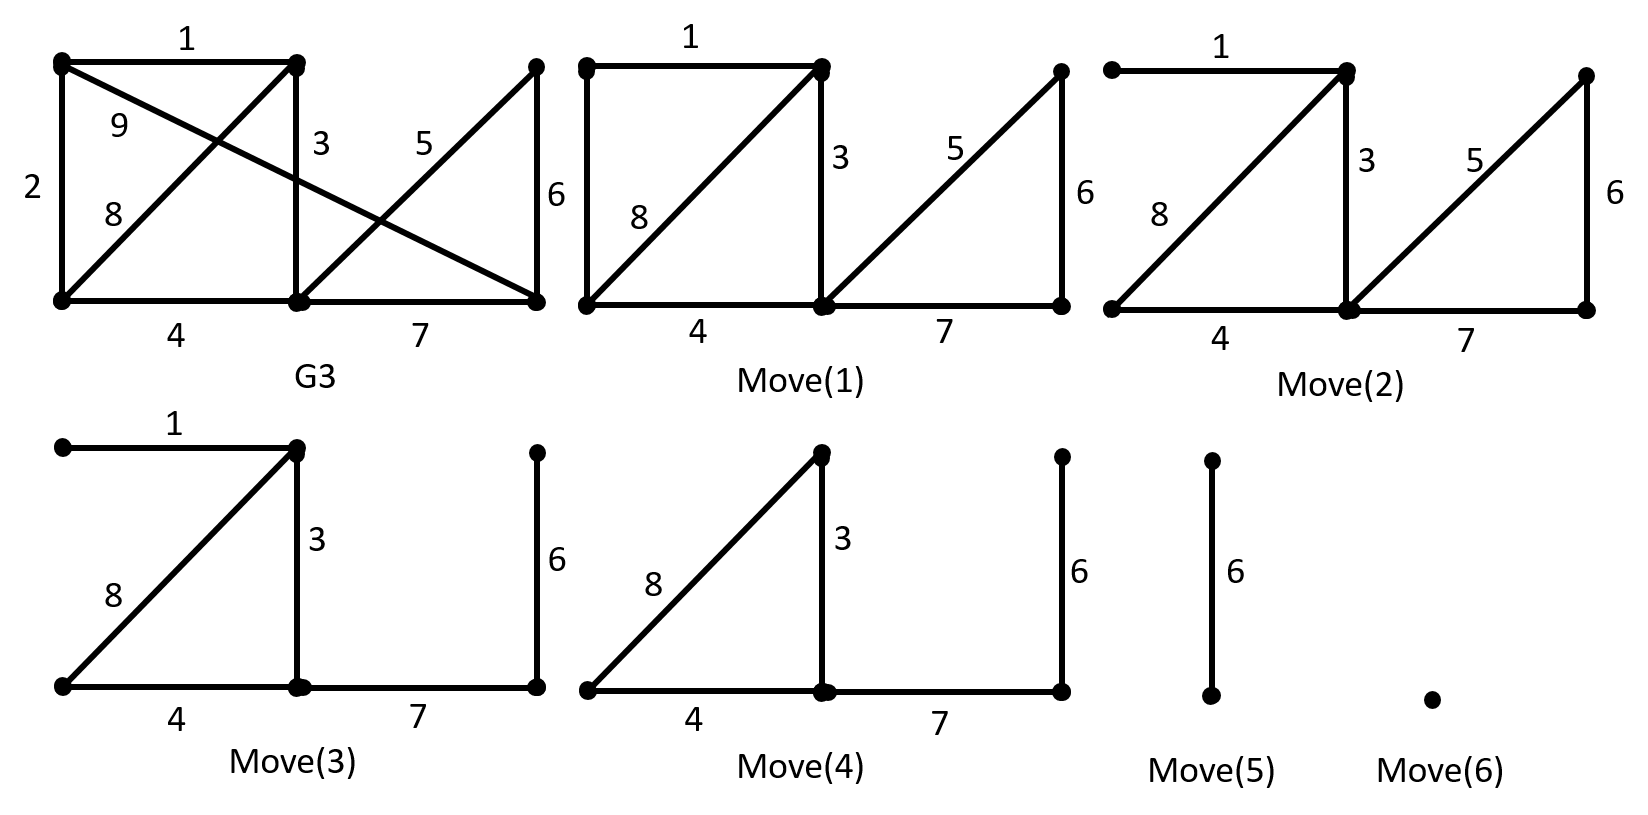
\includegraphics[scale =0.6]{g3.png}
      \caption{The hardness game for G3}
	  \label{fig:hd3}
      \end{center}
      \end{figure}
\end{examp}

%***************************************************************************************************************************************************************
%***************************************************************************************************************************************************************

\chapter{The Conflict Matrix of Multi-clause-sets}
\label{cha:The Conflict Matrix of Multi-clause-sets}
%--------------------------------------------------------------------------------------------------------------------------------------
\section{Definitions}
\label{sec:Definitions}

??????????????

\begin{defi}\label{def:dag}
      A \textbf{directed graph} (``dg'') is a pair $(V,E)$, where $V$ is a set (vertices), and $E \sse (V \times V) \sm \id_V$ 
	  (directed edges, not allowing loops). A \textbf{directed acyclic graph} (``dag'') is a dg $(V,E)$ without (directed) cycles.
\end{defi}


\begin{defi}\label{def:conflictmat}
A \textbf{conflict matrix} is a square matrix of order $m \in \NNZ$ with entries in $\NNZ$ and with zeros on the main diagonal 
(in other words, a conflict matrix is the adjacency matrix of some directed multigraph). A \textbf{symmetric conflict matrix} 
is a conflict matrix which is symmetric (in other words, symmetric conflict matrices are the adjacency matrices of multigraphs). 
Addition of (symmetric) conflict matrices yields again a (symmetric) conflict matrix.

 For $F \in \Mcls$ let \bmm{\scf(F)} be the \textbf{symmetric conflict matrix of} $F$, which is a square matrix of order $c(F)$ 
 with entries $\scf(F)_{i,j} := \abs{C_i \cap \ol{C_j}}$ (the number of literals $x \in C_i$ with $\ol{x} \in C_j$), where the 
 $C_i$ are the clauses of $F$ (in some order; with multiplicities). And let \bmm{\acf(F)} be the \textbf{asymmetric conflict matrix 
 of} $F$, a square matrix of order $c(F)$ with entries $\acf(F)_{i,j} := \abs{(C_i \cap \Va) \cap \ol{C_j}}$ (the number of positive 
 literals $x \in C_i$ with $\ol{x} \in C_j$)\cite{h14}.
\end{defi}
 Obviously $\scf(F)$ is a symmetric conflict matrix, while $\acf(F)$ is a conflict matrix, and we have \cite{h14}
\begin{displaymath}
  \scf(F) = \acf(F) + \acf(F)^t.
\end{displaymath}

%***************************************************************************************************************************************************************
%***************************************************************************************************************************************************************
\chapter{Autarkies}
\label{cha:Autarkies}
%--------------------------------------------------------------------------------------------------------------------------------------
\section{Autarkies}
\label{sec:Autarkies}

\begin{defi}\label{def:autarky1}
      A partial assignment $\vp \in \Pass$ is called an \textbf{autarky} for $F \in \Cls$ if $\fa\, C \in F : \vp * \set{C} \in \set{\set{C}, \top}$.
\end{defi}

Let $F$ be a clause-set. An autarky for $F$ is a partial assignment $\vp$ such that: $\fa C \in F : \var(\vp) \cap \var(C) \neq \es \Ra \vp * \set{C} = \top$ where $\vp * \set{C}$ is given by $\top$ when $\vp$ 
satisfies $\set{C}$, while otherwise $\vp * \set{C} = \set{C}$. 
Namely, whenever a clause is touched by a partial assignment $\vp$, then $\vp$ satisfies it.

\begin{defi}\label{def:weak autarky}
      A \textbf{weak autarky} ????????
\end{defi} 
\begin{lem}\label{lem:compaut}
      If $\vp, \psi$ are autarkies for $F$, then also the composition $\vp \circ \psi$ is an autarky for $F$.
\end{lem}
\pr If $\vp \circ \psi$ touches a clause $C \in F$ then either:
\begin{enumerate}
      \item $\psi$ touches $C$. Now, since $\psi$ is an autarky for $F, C$ is satisfied by $\vp \circ \psi$ since the assignments to variables in var($\psi$) 
	  do not  change and still exist in $\vp \circ \psi$. \item $\psi$ does not touch $C$ and $\vp$ therefore does touch C. Now, since $\vp$ is an autarky 
	  for $F$, C is satisfied by $\vp \circ \psi$ since the assignments to variables in $var(\vp) \cap var(C)$ for $\vp$ do not change in $\vp \circ \psi$. 
\end{enumerate}
Remarks:
\begin{enumerate}
      \item The empty partial assignment $\epa$ is an autarky for every $F \in \Cls$ (no clause is touched), and more generally all $\varphi \in \Pass$ with $\var(\varphi) \cap \var(F) = \emptyset$
      are autarkies for $F$, the textbf{trivial autarkies}. On the other end of the spectrum every satisfying assignment for $F$ (i.e., $\varphi * F = \top $) is an autarky for $F$ 
	  (every clause is satisfied). A literal $x \in \Lit$ is a pure literal for $F$ iff $\langle x \rightarrow 1 \rangle $ is an autarky for $F$ \cite{h9}.
\end{enumerate}
\begin{examp}\label{exp:autarky1} 
      For $F \in \Cls$ and $F=\{ \{a,b\}, \{ \neg a, c\}\}$ the two partial assignments $\langle b \rightarrow 1 \rangle$ and 
	  $\langle c \rightarrow 1 \rangle$ are autarkies. Also, $\langle a \rightarrow 1, c \rightarrow 1  \rangle$, 
	  $\langle a \rightarrow 0, b \rightarrow 1  \rangle$ and $\langle b \rightarrow 1, c \rightarrow 1  \rangle$ are autarkies 
	  for $F$. But, $\langle b \rightarrow 0 \rangle$, $\langle c \rightarrow 0 \rangle$ and $\langle a \rightarrow 1 \rangle$ 
	  are not autarkies for $F$.
\end{exam}
%----------------------------------------------------------------------------------------------------------------------
\section{Hitting clause-sets}
\label{sec:hitting}

\begin{defi}\label{def:hitting}
      A \textbf{hitting clause-set} is an $F \in \Cls$ such that all $C, D \in F$, $C \ne D$, have a clash, i.e, $C \cap \ol{D} \ne \es$ holds; 
	  the set of all hitting clause-sets is denoted by $\bmm{\Clash} \subset \Cls$, while $\bmm{\Uclash} := \Clash \cap \Usat$.
\end{defi}
Remarks:
\begin{enumerate}
      \item For $C, D \in \Cl$ the following properties are equivalent (recall Lemma \ref{lem:comcomp}):
      \begin{enumerate}
            \item $C, D$ clash, that is, there are clashing literals $x \in C$, $y \in D$.
            \item $C \cap \ol{D} \ne \es$.
            \item $\ol{C} \cap D \ne \es$.
            \item $C \cup D \ne \Cl$.
      \end{enumerate}
      \item $F \in \Cls$ is hitting iff every $C \in F$, as partial assignment, is a satisfying assignment for $F \sm \set{C}$.
\end{enumerate}
\begin{examp}\label{exp:hit1} 
      We have e.g. $\{1, 2,-3 \} \in \Cl$, while $\{-1, 1\} \not \in \Cl$. The only clause-set in $\Clash$ containing the empty clause is $\{ \bot \} \in \Clash$ . 
	  An example of a non-hitting clause-set is $\{ \{ 1, 2\}, \{-1, 2\}, \{3 \} \} \in \Cls \setminus \Clash$ , where we obtain an element of $\Clash$ if we add 
	  literal $-2$ to the third clause \cite{h9}.
\end{exam}
\begin{examp}\label{exp:hit2} 
      ????????????
	 $ \{\{a,b,c\},\{ \overbar a, \overbar b \},{a, \overbar c \}\}$ is a hitting clause-set
\end{exam}

\begin{examp}\label{exp:hit}
  $\top \in \Sat \cap \Clash$ and $\set{\bot} \in \Uclash$. In general a full clause-set $F$ is unsatisfiable iff 
  $F = A(\var(F))$), and thus $A(V) \in \Uclash$ for all finite $V \subset \Va$.

  The fundamental property for $F \in \Clash$: Consider $\vp, \psi \in \Pass$, such that there are $C, D \in F$, 
  $C \ne D$, with $\vp * \set{C} = \psi * \set{D} = \set{\bot}$ (that is, $\bot \in \vp * F \cap \psi * F$, where there are different falsified clauses for these two partial assignments). Then $\vp, \psi$ are incompatible, i.e., there is $v \in \var(\vp) \cap \var(\psi)$ with $\vp(v) \ne \psi(v)$.

  It follows easily that for $F \in \Clash$ holds $F \in \Usat \Lra \sum_{C \in F} 2^{-\abs{C}} = 1$ \cite{h9}.
\end{examp}


\begin{defi}\label{def:hitting2}
       A \textbf{k-uniform hitting clause-set} is a hitting clauseset F such that for all clauses C1;C2 2 F, C1 6= C2 we
have jC1 \C2j = k, and a uniform hitting clause-set is a k-uniform hitting clause-set for some k.
The above
example is not a uniform hitting clause-set, while $ \{\{a,b,c\},\{ \overbar a, b \},{a, \overbar c \}\}$ is a 1-uniform hitting clause-set.
???????????????
\end{defi}
\begin{defi}\label{def:nearlyhitting}
      A \textbf{nearly-hitting clause-set} is an $F \in \Cls$, such that for all $C, D \in F$, $C \ne D$ either $\var(C) \cap \var(D) = \es$ holds or $C, D$ 
	  have a clash; the set of all nearly-hitting clause-sets is denoted by $\bmm{\Nclash} \subset \Cls$.
\end{defi}
Remarks:
\begin{enumerate}
      \item $F \in \Cls$ is nearly-hitting iff every $C \in F$, as partial assignment, is an autarky for $F \sm \set{C}$.
\end{enumerate}

\begin{quest}\label{que:decisionnearlyhitting}
      The complexity of SAT-decision for nearly-hitting clause-sets is open (also in the boolean case).
\end{quest}

%--------------------------------------------------------------------------------------------------------------------------------------
\section{Deficiency}
\label{sec:Deficiency}

A very interesting measure for the complexity of formulas is $CNF$ is the so-called "deficiency" which indicates the difference 
between the number of clauses and the number of variables.
\begin{defi}\label{def:df1}
      Let $F$ be a formula in $CNF$ with $n$ clauses and $k$ variables. Then, the \textbf{deficiency} of $F$ is defined as $\delta (F) = n - k$. 
	  Further, we define the maximal deficiency as $\delta ^*(F) = \max \{ \delta (G) \mid G \subseteq F \}$ \cite{h6}.
\end{defi} 
Let $k-CNF$ be the set of $CNF$-formulas with deficiency (exactly) $k$. Then, the satisfiability problem for $k-CNF$ is NP-complete. 
Similarly, let $CNF ^* (k)$ be the set of formulas with maximal deficiency $k$, i.e. 
$\{F \in CNF : \delta ^*(F) = k \}$. It can been shown that the satisfiability problem for these classes is solvable in polynomial time \cite{h6}.

%----------------------------------------------------------------------------------------------------------------------
\section{Minimal Unsatisfiability}
\label{sec:minsat}

\begin{defi}\label{def:minsat1}
      An unsatisfiable clause-set F is called \textbf{minimally unsatisfiable}, if for every clause $C \in F$ the clause-set $F \setminus \{C\}$ 
	  is satisfiable, and the set of minimally unsatisfiable clause-sets is denoted by $\bmm{\Musat} \subset \Usat$ . A clause-set $F \in \Musat$ is called
	  \textbf{saturated}, if replacing any $C \in F$ by any super-clause $C' \supset C$ yields a satisfiable clause-set, and the set of saturated 
	  minimally unsatisfiable clause-sets is denoted by $\Smusat \subset \Musat$.
\end{defi}
%\begin{examp}\label{exp:minsat1} 
%      The simplest element of $\Usat \setminus \Musat$ is $\{ \bot, \{ 1\} \}$, while the simplest element of $\Musat \setminus \Smusat$ is $\{ \{1, 2\}, \{-1\}, \{-2\} \}$ \cite{h9}.
%\end{exam}	  
%--------------------------------------------------------------------------------------------------------------------------------------
\newpage
\bibliography{HA_ResearchRef}
\bibliographystyle{plainurl}


\end{document}

